\chapter{Results}\label{sec:results}

\section{Base case} \label{sec:base_case}
As a reference for all following calculations, a model representing the Blennerhassett Island Bridge's final design is investigated. The results obtained by the analysis are then compared to the ones in the design drawings for plausibility. A particular challenge is the determination of the self-equilibrium stress state. As the arch was defined as an unsuitable parabola, appropriate hanger forces were determined by trial and error in the design. These permanent hanger forces of the final design are available in the drawings. However, they are inadequate for calculating the base case, as the load distribution in the model is simplified. Instead of another trial and error procedure for the base case, the hanger forces are obtained as the result of a simultaneous arch and tie moment optimisation. Thereby, the arch's moment is weighed by a factor of 1.5 to achieve an optimal similarity. Further, the hanger forces are bounded between 25\% and 45\% of their nominal strength. The base case's internal force distributions for the permanent state are shown in \cref{fig:base_case_permanent}. Instead of the normal force in the hangers, the demand over capacity ratio is shown directly. Only the hangers of one set are shown, namely the ones inclined to the right side, and the dots are connected for readability. As a comparison, the extreme values of each component, which are found in the design verifications in Appendix \ref{app:design_verifications}, are also shown.

\begin{figure}[H]
    \centering
    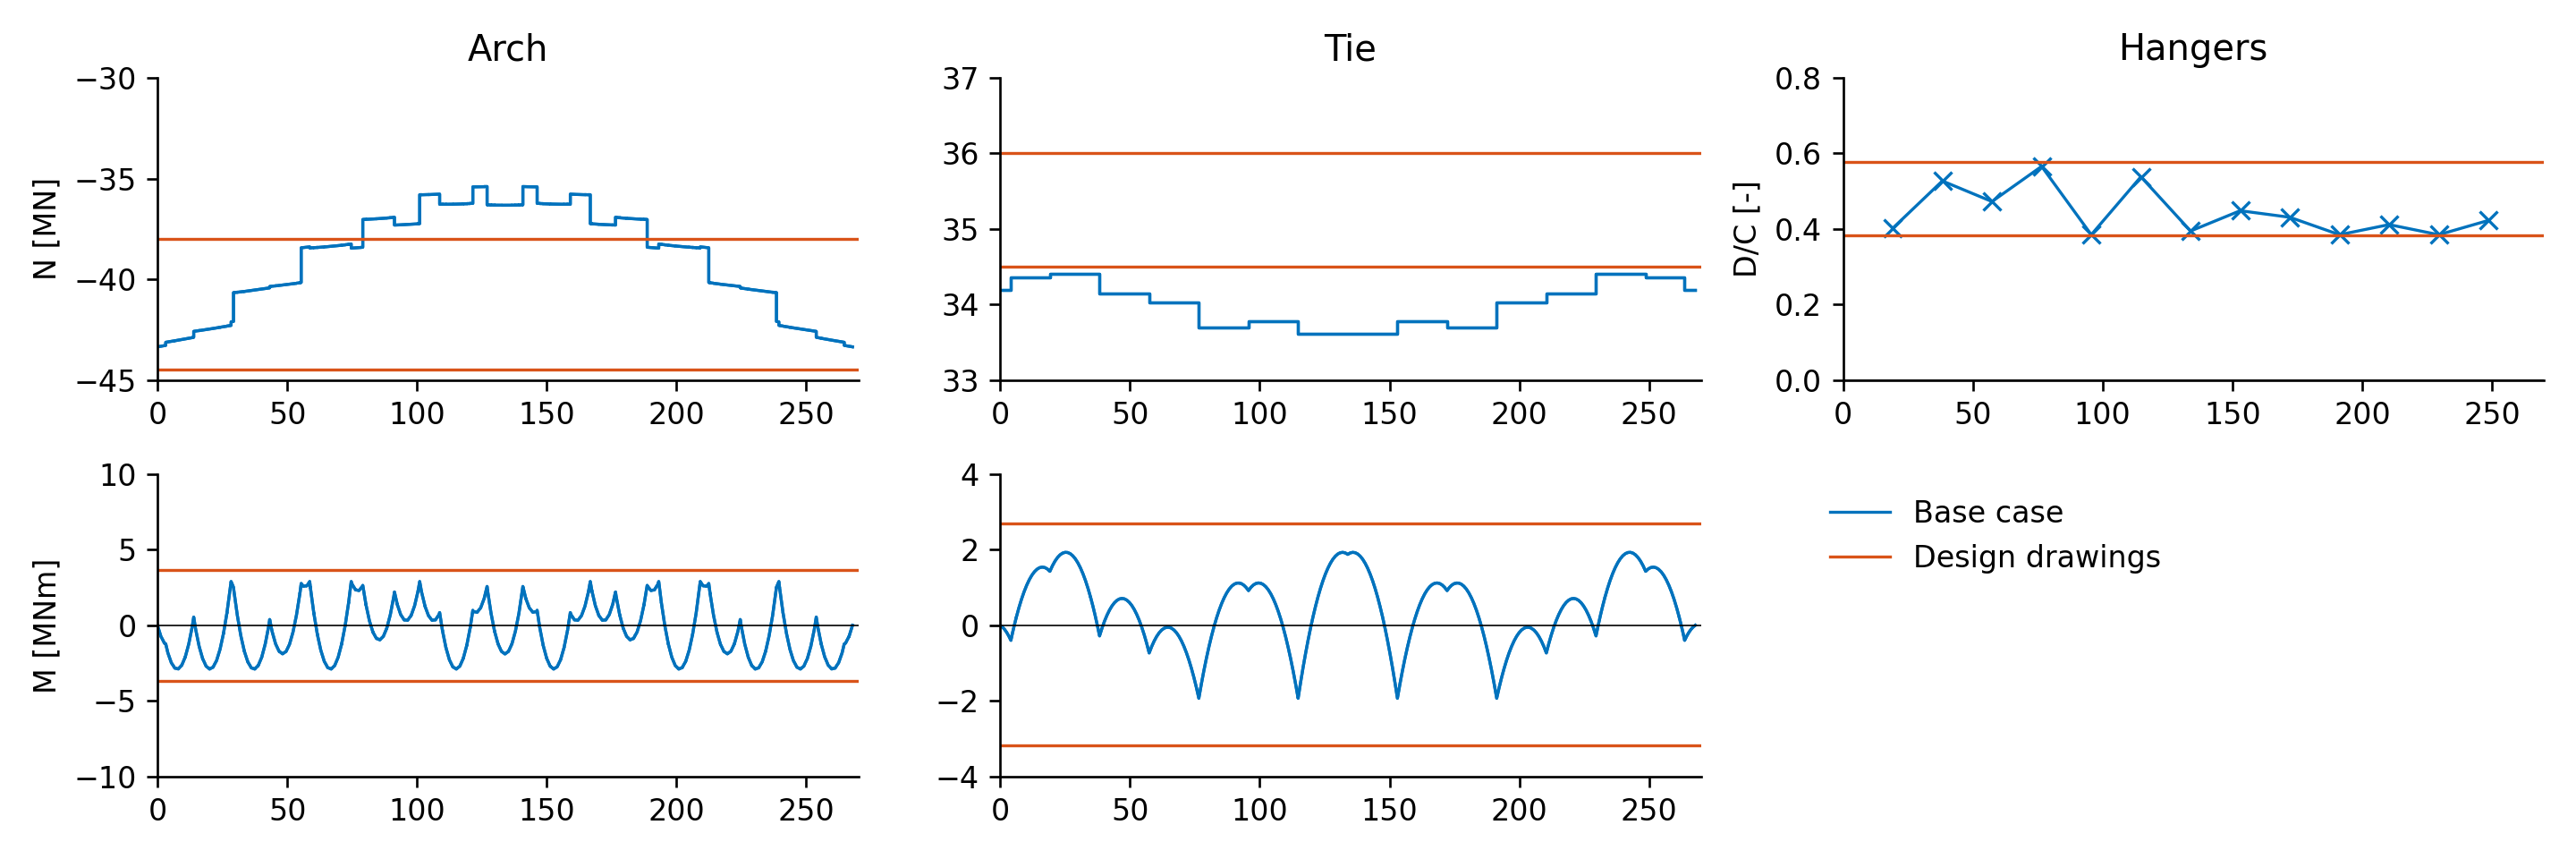
\includegraphics[width=\textwidth]{calculations/Base case/Permanent state.png}
    \caption{Permanent internal forces of the base case and reference values from the drawings}
    \label{fig:base_case_permanent}
\end{figure}

The moment distributions in the arch and the tie, as well as the normal forces in the hangers, match the design drawings very well. Only for the normal force in the arch rib and the tie girder an offset of \SI{2}{MN} can be observed. This difference is probably due to underestimating the weight of the bridge and because of its simplified assignment to the beam elements. However, overall the obtained internal force distribution matches the design drawings sufficiently well. Further, It can be concluded, that for a fixed arch shape the simultaneous arch and tie moment optimisation yields adequate results. Another comparison is drawn between the effects under characteristic live loads. As there are countless live load combinations, which are to be accounted for, it makes sense to look at the entire range of possible internal forces. They are shown in \cref{fig:base_case_live} by the two blue lines representing the lower and the upper limit. These ranges are compared to the values specified in the design verifications of the design drawings.

\begin{figure}[H]
    \centering
    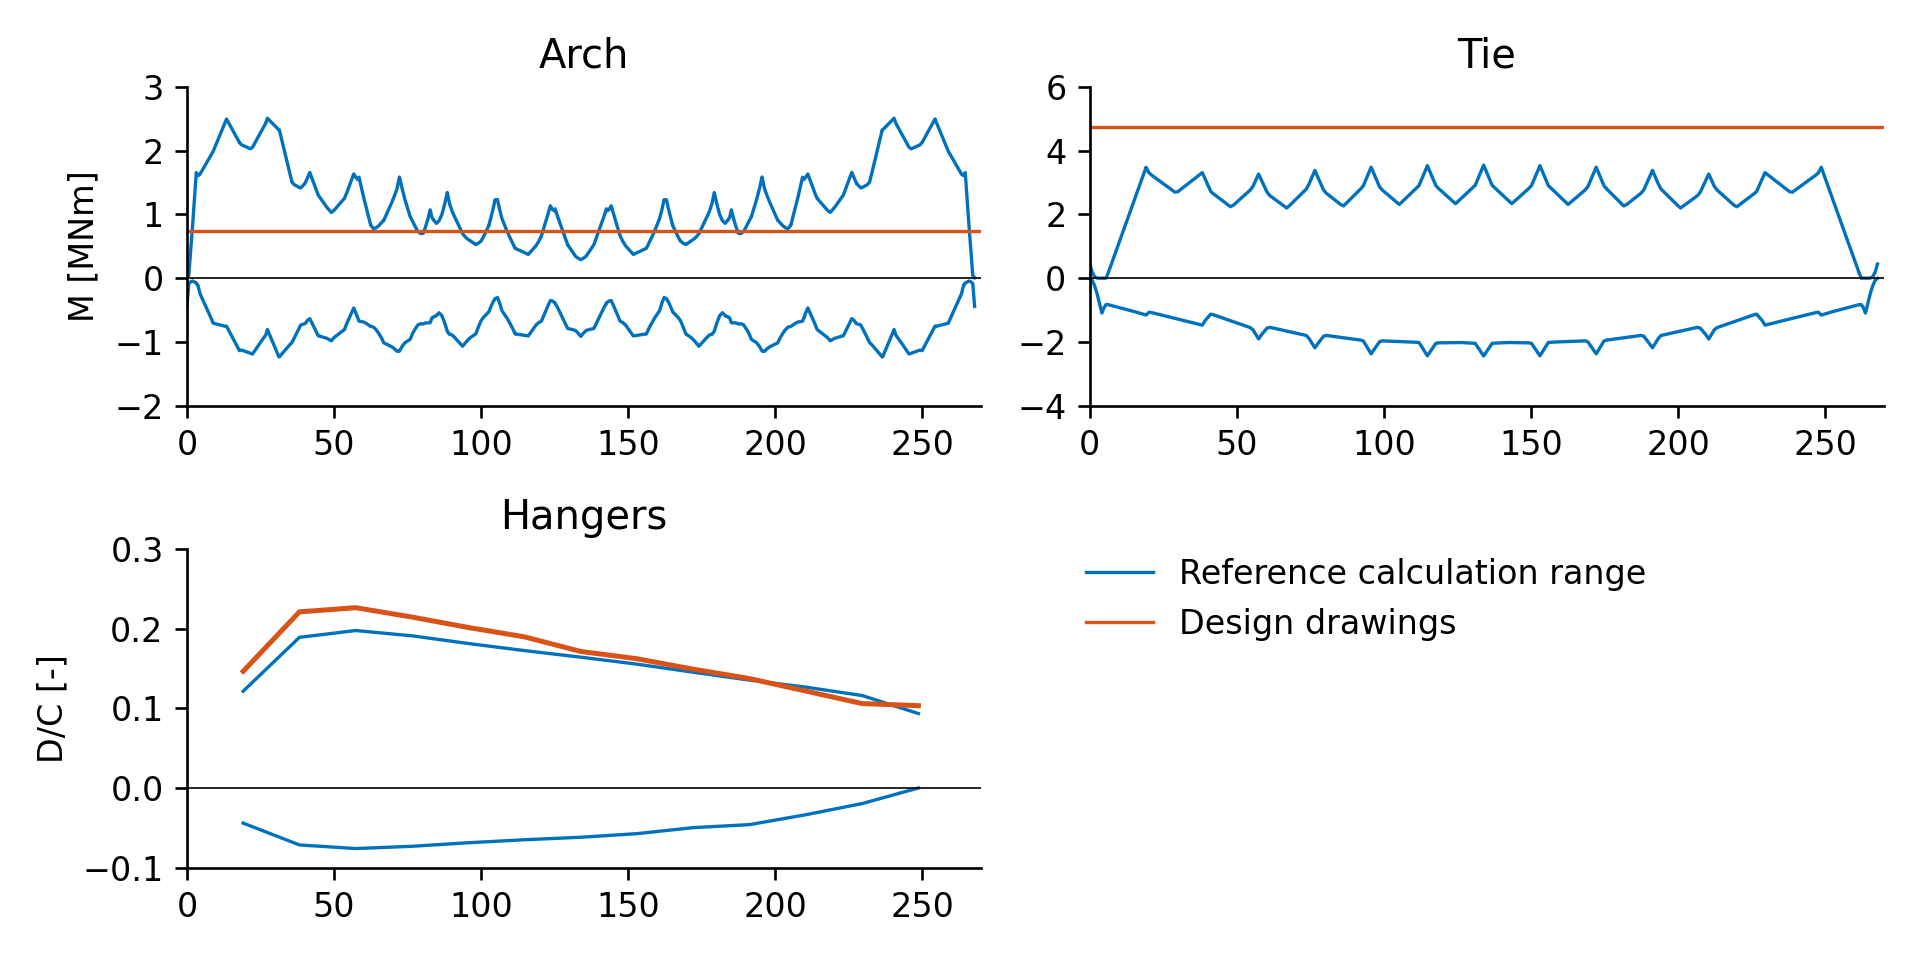
\includegraphics[width=0.8\textwidth]{calculations/Base case/Live load.png}
    \caption{Range of internal forces effects under live loading}
    \label{fig:base_case_live}
\end{figure}

The moment distribution in the arch shows a a significant offset to the value given in the design drawings. However, it is impossible that this value represents the maximum moment under live loading, considering the given hanger forces. Therefore, this difference is ignored. The moment distribution in the tie and the hangers' normal forces agree well on the other hand. Apparently, the live loading is only slightly overestimated in the model, which can be seen particularly well in the hangers' demand over capacity ratios. These differences are accepted, as it is not the goal of this Thesis to reproduce the results from the design drawings. Interestingly, in particular, the arch segment near the knuckle is affected by strong bending moments. In the tie girder on the other hand, the range of effects under live loading is well distributed. Apparently, the influence lines for the moments in the tie girder at the different cross-girders roughly follow the same shape. For the hangers, it is the second one from the knuckle connected toward the middle of the arch that undergoes the largest normal force. Towards the other side of the hanger set, the hanger forces decrease. The strongly affected hangers have in common that their inclination is closer to the arch's inclination at their respective connection node. The arch is very stiff on axial loading and comparably weaker on perpendicular forces. Therefore, at the arch nodes, smaller displacements in the hanger's direction are expected for the first hangers of the considered hanger set, explaining their higher normal forces. Only the first hanger does not follow this rule, which is explained by its smaller area of influence due to the nearby knuckle. \medskip

The resulting demand over capacity ratios for all segments and limit states are presented in Table \ref{tab:dc_base_case}. Considering the strength limit states, wind exposure is governing for the segment close to the knuckle for both the arch and the tie. For the segment in the field, as well as for the hangers, it is the vehicular load which poses the highest demand. The limit state for high dead-to-live load ratios is not decisive for any segment. A comparison to the ratios found in the design drawings, presented in Table \ref{tab:dc_drawings}, shows that this is not the case for the final design. The underestimation of the demand of the strength-IV limit state is probably due to a general underestimation of the weight, which has already been seen for the permanent effects. Nonetheless, the strength limit states agree well with the verifications found in the design drawings, even though slightly underestimated. For cable loss and replacement on the other hand, the demands predicted by the considered model are overestimated. Besides the higher dynamic amplification factors of 1.75, this is due to the modelling of a single arch plane, which does not take into account the other undamaged arch plane. Nevertheless, the results are within an acceptable range. For the tie fracture extreme event, which is considered in a simplistic manner, demands near 1.00 result. This agrees with the design drawings, in which it is only noted that the tie fracture governed the design of the tie girder. For the comparative investigations in this Thesis the simplistic verification is adequate, as the tendencies can be modelled sufficiently accurate.

\begin{table}
    \centering
    \caption{Demand over capacity ratios of the base case}
    \label{tab:dc_base_case}
    \input{calculations/Base case/dc table.txt}
\end{table}

\begin{table}[H]
    \centering
    \caption{Demand over capacity ratios of the final design}
    \label{tab:dc_drawings}
    \begin{tabular}{lccccccc}
    \toprule
    Segment & \multicolumn{7}{c}{Demand / Capacity} \\
     & S-I & S-III & S-IV & Replacement & Loss & Fracture & Fatigue\\ \midrule 
    Arch 1 & - & \textbf{1.00} & - & - & 0.85 & -  & - \\ 
    Arch 2 & - & - & 0.99 & - & \textbf{1.00} & -  & - \\ 
    Arch 3 &  - & - & 0.83 & - & \textbf{0.97} & -  & - \\ 
    Tie 1 & - & 0.69 & - & - & 0.61 & $\sim$\textbf{1.00} & - \\ 
    Tie 2 & 0.68 & - & - & - & 0.88 & $\sim$\textbf{1.00} & - \\ 
    Tie 3 & 0.63 & - & - & - & 0.76 & $\sim$\textbf{1.00} & - \\ 
    Hangers & 0.91 & 0.77 & 0.75 & - & 0.74 & -  & -\\ 
    \bottomrule
\end{tabular}

\end{table}

\newpage
\section{Arch shape} \label{sec:arch_shape}
In this section, the arch shape is first investigated individually as it affects the investigation of the following hanger-related design variables. Most network tied-arch bridges feature a parabolic arch. It is a relic of the classical tied-arch bridge with vertical hangers. 
The vertical hanger forces on the arch are evenly distributed and the respective thrust line approximately matches the parabola, if the arch weight is negligible.
For network tied-arch bridges, circular arch shapes have been considered suitable for radial arrangements. Each pair of radial hangers equals an approximately radial loading which causes a circular thrust line.
For a rise to span ratio of $r/s=0.2$, the two shapes diverge by up to 0.8\% of the span. While this differences might seem negligible on a drawing, the impact of this difference on the arch's moment distribution is significant, as it is bigger than its usual cross-section height. 
The implications are first investigated on the Blennerhassett Island Bridge in \cref{sec:arch_shape_BIB}. Afterwards, the arch shapes are studied for a denser and a continuous hanger arrangement in \cref{sec:arch_shape_increased} and \cref{sec:arch_shape_continuous}. The extreme event of cable loss is disregarded for in this investigation, because its impact on the design verifications depends much more on the hanger arrangement than on the arch shape.

\subsection{Blennerhassett Island Bridge} \label{sec:arch_shape_BIB}
The typical solution to the issue of the arch shape's deviation from the thrust line is the assignment of non-uniform permanent hanger forces resulting in a thrust line similar to the arch shape. However, adapting the arch shape to the thrust line can be considered a more elegant solution. 
Multiple approaches to determine the arch shape have been introduced in Section \ref{sec:met_arch}. All of them are linked to the thrust line, which is the most efficient shape. The following four arch shapes are compared in this investigation.
\begin{enumerate}
    \item Thrust line: This shape is obtained numerically, as described in \cref{sec:discrete}, as the thrust line for the uniform hanger forces obtained from a tie moment optimisation. The respective hanger forces are equal to $N_p=\SI{1.8}{MN}$ corresponding to 28\% of their nominal resistance.
    \item Polynomial thrust line approximation: The above thrust line is approximated by a quartic function. The quartic function is obtained according to \cref{sec:polynomial_approximation} using the shape parameter $b$. This parameter is obtained by a least squares approximation. 

    \item Spline thrust line approximation: As a second approximation of the thrust line a cubic spline defined by the respective arch-hanger connection nodes is used. These nodes are therefore represented at their exact location. The shape is characterised by a continuous curvature.
    \item Thrust line of continuous hanger arrangement: This shape is the thrust line of the hypothetical continuous hanger arrangement, which was introduced in \cref{sec:continuous}.
\end{enumerate}

To make their differences visible, the respective deviations to the parabolic shape are shown in \cref{fig:arch_shapes_13}. 
%Also a circular arch is shown to put the results into perspective.

\begin{figure}[H]
    \centering
    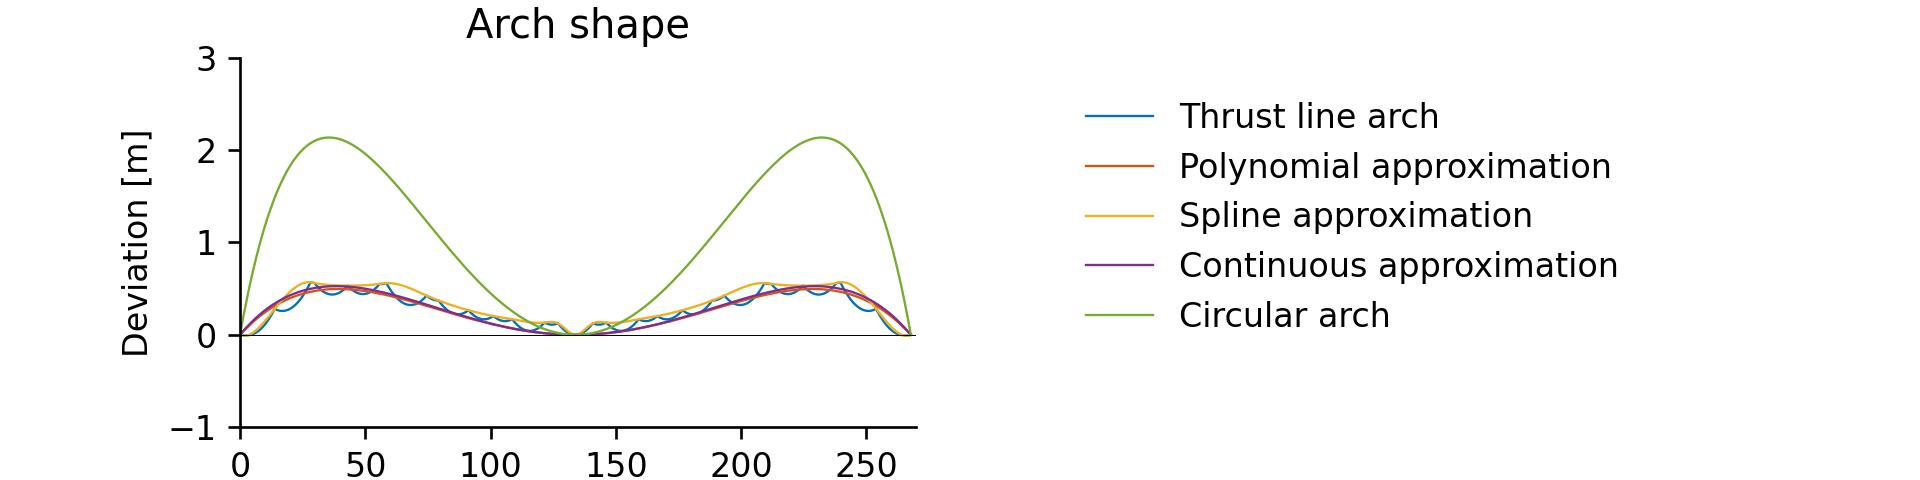
\includegraphics[trim={1cm 0 3cm 0},clip, width=0.76\textwidth]{calculations/arch shape/arch_shapes_13.png}
    \caption{Deviation of arch shapes to the parabola}
    \label{fig:arch_shapes_13}
\end{figure}

In the range between the circular and the parabolic shape, the thrust line tends slightly to the parabolic side. All three approximations seem to fit the thrust line reasonably well. But to investigate the impacts of the remain deviations from the thrust line, the corresponding permanent moment distribution is presented in \cref{fig:arch_permanent_moments_13}. Further, from the similarity between the polynomial and the continuous approximation, it can be concluded, that if the hanger arrangement is dense enough, a quartic function can yield an appropriate arch shape for this hanger arrangement pattern. 

\begin{figure}[H]
    \centering
    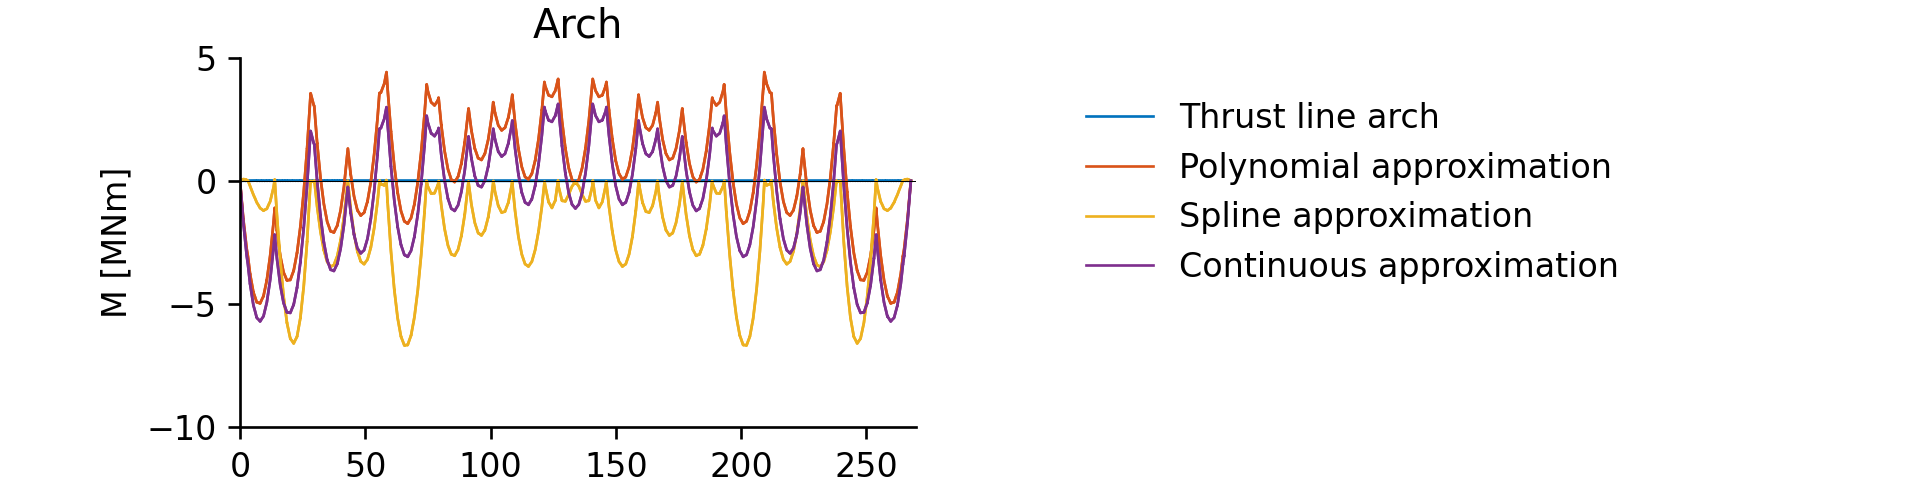
\includegraphics[trim={1cm 0 3cm 0},clip, width=0.76\textwidth]{calculations/arch shape/permanent state_13.png}
    \caption{Permanent arch moment distributions depending on arch shape}
    \label{fig:arch_permanent_moments_13}
\end{figure}

Despite the apparent match of the arch shapes, significant bending moments result in each of the three approximations. The spline approximation's moment distribution is strictly negative, which relies on the characteristic that a spline lies above the approximately linear thrust line and only matches it at the connection nodes. It is particularly interesting, that all approximations feature a similar parabolic moment distribution between the arch-hanger connection nodes. While these moment distributions resulting for the approximated shapes are certainly considerable, it is infeasible to find a convex shape matching the arch thrust line. Any shape with an approximately constant radius $R$ between two nodes results in a deviation from the approximately linear thrust line and causes the corresponding deviation moment $\Delta M$. This deviation can be approximated depending on the distance between two hanger connection nodes $d$ and the arch's normal force $N$ according to \cref{eq:moment_deviation}.

\begin{equation}
    \Delta M=-\left(R-\sqrt{R^2-\left(d/2\right)^2}\right) \cdot N
    \label{eq:moment_deviation}
\end{equation}

For the Blennerhassett Island Bridge, these variables roughly correspond to $R=\SI{194}{m}$, $d=\SI{17}{m}$ and $N=\SI{40}{MN}$. Equation \eqref{eq:moment_deviation} yields a deviation moment of $\Delta M=\SI{7.5}{MNm}$ coming close to the value observed in \cref{fig:arch_permanent_moments_13}. From the analytical form of Equation \eqref{eq:moment_deviation} it can further be concluded, that a reduction of the hanger node spacing has a more than proportional impact on the bending deviation moment. From this perspective, an optimum hanger arrangement features one hanger per connection node and a uniform spacing on the arch. The minimum spacing can thereby be reduced to $d=\SI{11}{m}$ and the deviation moment to $\Delta M=\SI{3.1}{MNm}$
To put these deviations into the context of the design verifications, the demand over capacity ratios resulting in the arch are shown in Table \ref{tab:arch_shape_dc_13} along with the decisive limit state.

\begin{table}[H]
    \centering
    \caption{Arch design verifications for different arch shapes}
    \label{tab:arch_shape_dc_13}
    \input{calculations/arch shape/dc_comparison_13.txt}
\end{table}

The deviations from the thrust line of the considered arch shapes increase the demand over capacity ratios by 0.06 on average. This difference is not critical for the initial design, but it offers some potential for optimisation. Further, it should be noted that also the exact thrust line is not the most efficient arch shape. In the strength limit state for vehicular use, the arch is affected by stronger positive bending moments than negative ones, as shown in \cref{fig:arch_shape_strength_1}. Therefore, a certain upward deviation from the thrust line and the resulting negative bending moment can prove beneficial to the verifications. This potential was estimated by evaluating the difference of the maximum and minimum bending moments in the decisive limit state and comparing it to the resistance. The comparison yielded possible reductions of the D/C ratio for the three segments between 0.01 and 0.03.

\begin{figure}[H]
    \centering
    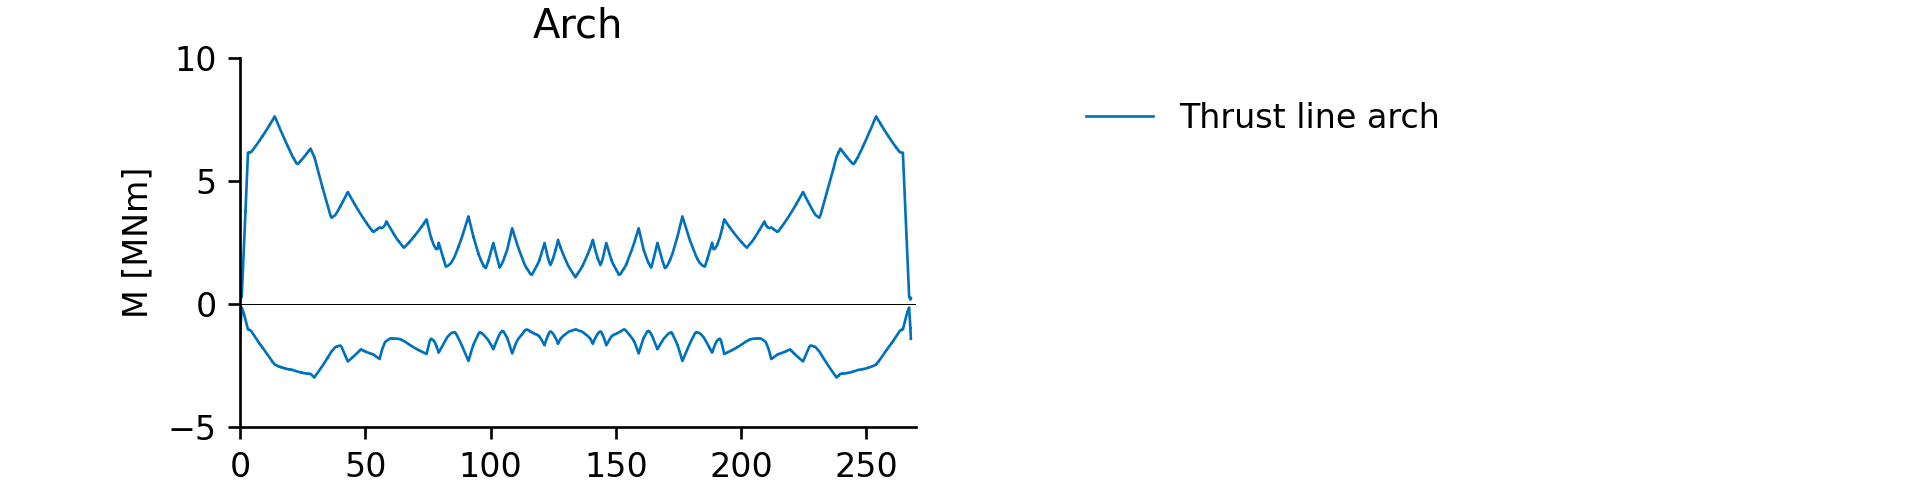
\includegraphics[trim={1cm 0 3cm 0},clip, width=0.76\textwidth]{calculations/arch shape/strength-I_13.png}
    \caption{Range of moments in the strength-I limit state}
    \label{fig:arch_shape_strength_1}
\end{figure}

\subsection{Increased hanger density} \label{sec:arch_shape_increased}
Ultimately, the influence of the hanger density on the arch shape is investigated. It was concluded from Equation \eqref{eq:moment_deviation}, that by reducing the distances between the hangers an over-proportional reduction in the permanent moment distribution results. Therefore, a similar calculation of the four arch shapes with 26 hangers per set was conducted. The resulting arch shapes are presented in \cref{fig:arch_shapes_26}.

\begin{figure}[H]
    \centering
    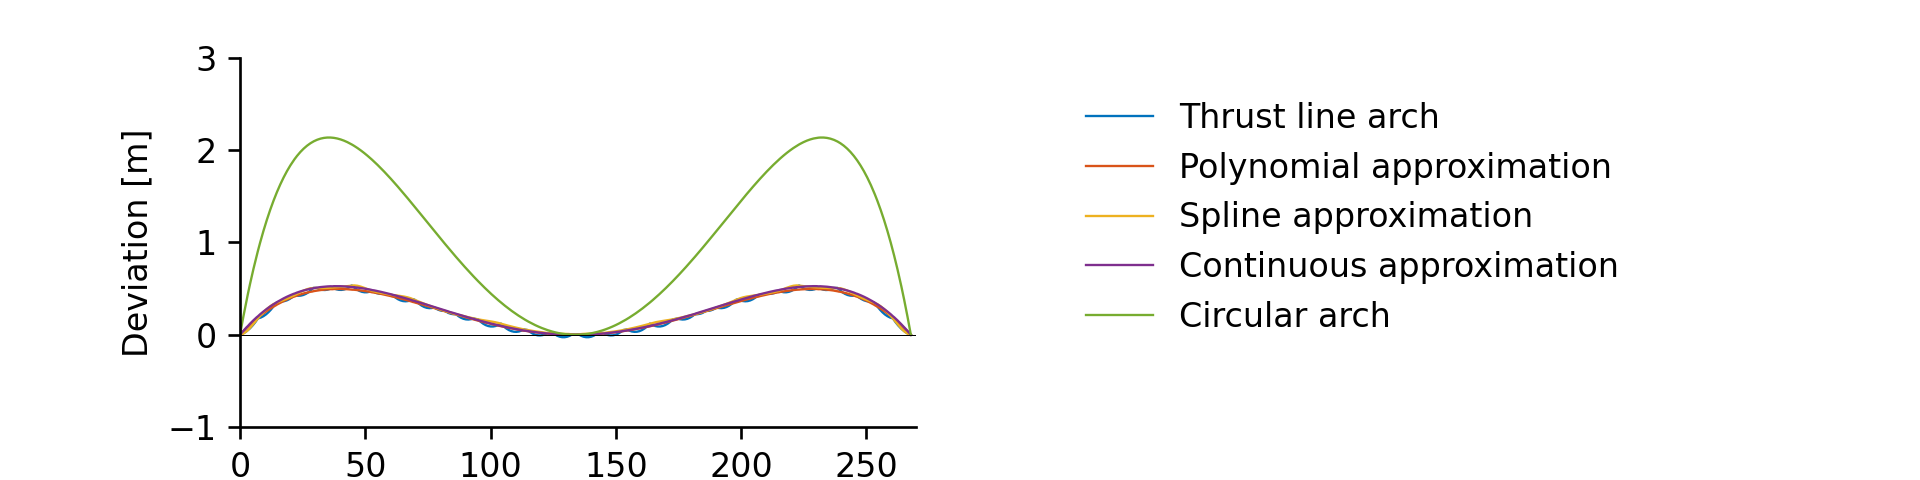
\includegraphics[trim={1cm 0 3cm 0},clip, width=0.76\textwidth]{calculations/arch shape/arch_shapes_26.png}
    \caption{Deviation of arch shapes from parabolic shape (26 hangers)}
    \label{fig:arch_shapes_26}
\end{figure}

If the amount of hangers is large enough, all considered approximations yield suitable arch shapes. The impact of the remaining deviation from the thrust line on the design verifications is negligible, as can be seen in the uniform demand over capacity ratios presented in Table \ref{tab:arch_shape_dc_26}. For the initial design, especially the continuous approximation presents a promising arch shape, as it does not involve a specific thrust line calculation. However, for sparse hanger arrangements, a more accurate modelling of the thrust line, involving the characteristic kinks, might be inevitable for the arch shape.

\begin{table}[H]
    \centering
    \input{calculations/arch shape/dc_comparison_26.txt}
    \caption{Arch design verifications (26 hangers)}
    \label{tab:arch_shape_dc_26}
\end{table}

\subsection{Continuous hanger arrangement} \label{sec:arch_shape_continuous}


\newpage
\section{Hanger density}
A denser hanger arrangement provides multiple benefits. As seen in the previous chapter, the shape deviation moments are reduced through the corresponding reduction of the distances between the hangers' anchorages. Further, the effects in the extreme event of cable loss are significantly lowered, as the hanger forces are reduced with the increase of hangers. Also the impaired structural system loses less of its essential stiffness and undergoes additionally lower effects therefore. However, the challenging task is to find an appropriate self-equilibrium stress state for structural systems in which the locations of the floor beams and the hangers do not coincide on the tie girder. 
In this investigation, this challenge is tackled by tie moment optimisation method. It allows finding the permanent hanger forces within a certain range, minimising the resulting moment distribution in the tie girder. This range is set between 25\% and 40\% of the hangers' characteristic capacity.  Four bridges are analysed featuring 13, 20, 26 or 27 hangers per set and a constant number of 13 floor beams. The arch shapes are defined as the quartic polynomial approximation of the thrust line. The model featuring 26 hangers is shown in \cref{fig:structure_26}. The spacing between the knuckle and the first hanger is slightly increased so there is an equally spaced pair of hangers around every floor beam. While the arrangement appears dense, the hanger spacing on the tie girder is still around \SI{10}{m} representing a rather high value for modern network tied-arch bridges.

\begin{figure}[H]
    \centering
    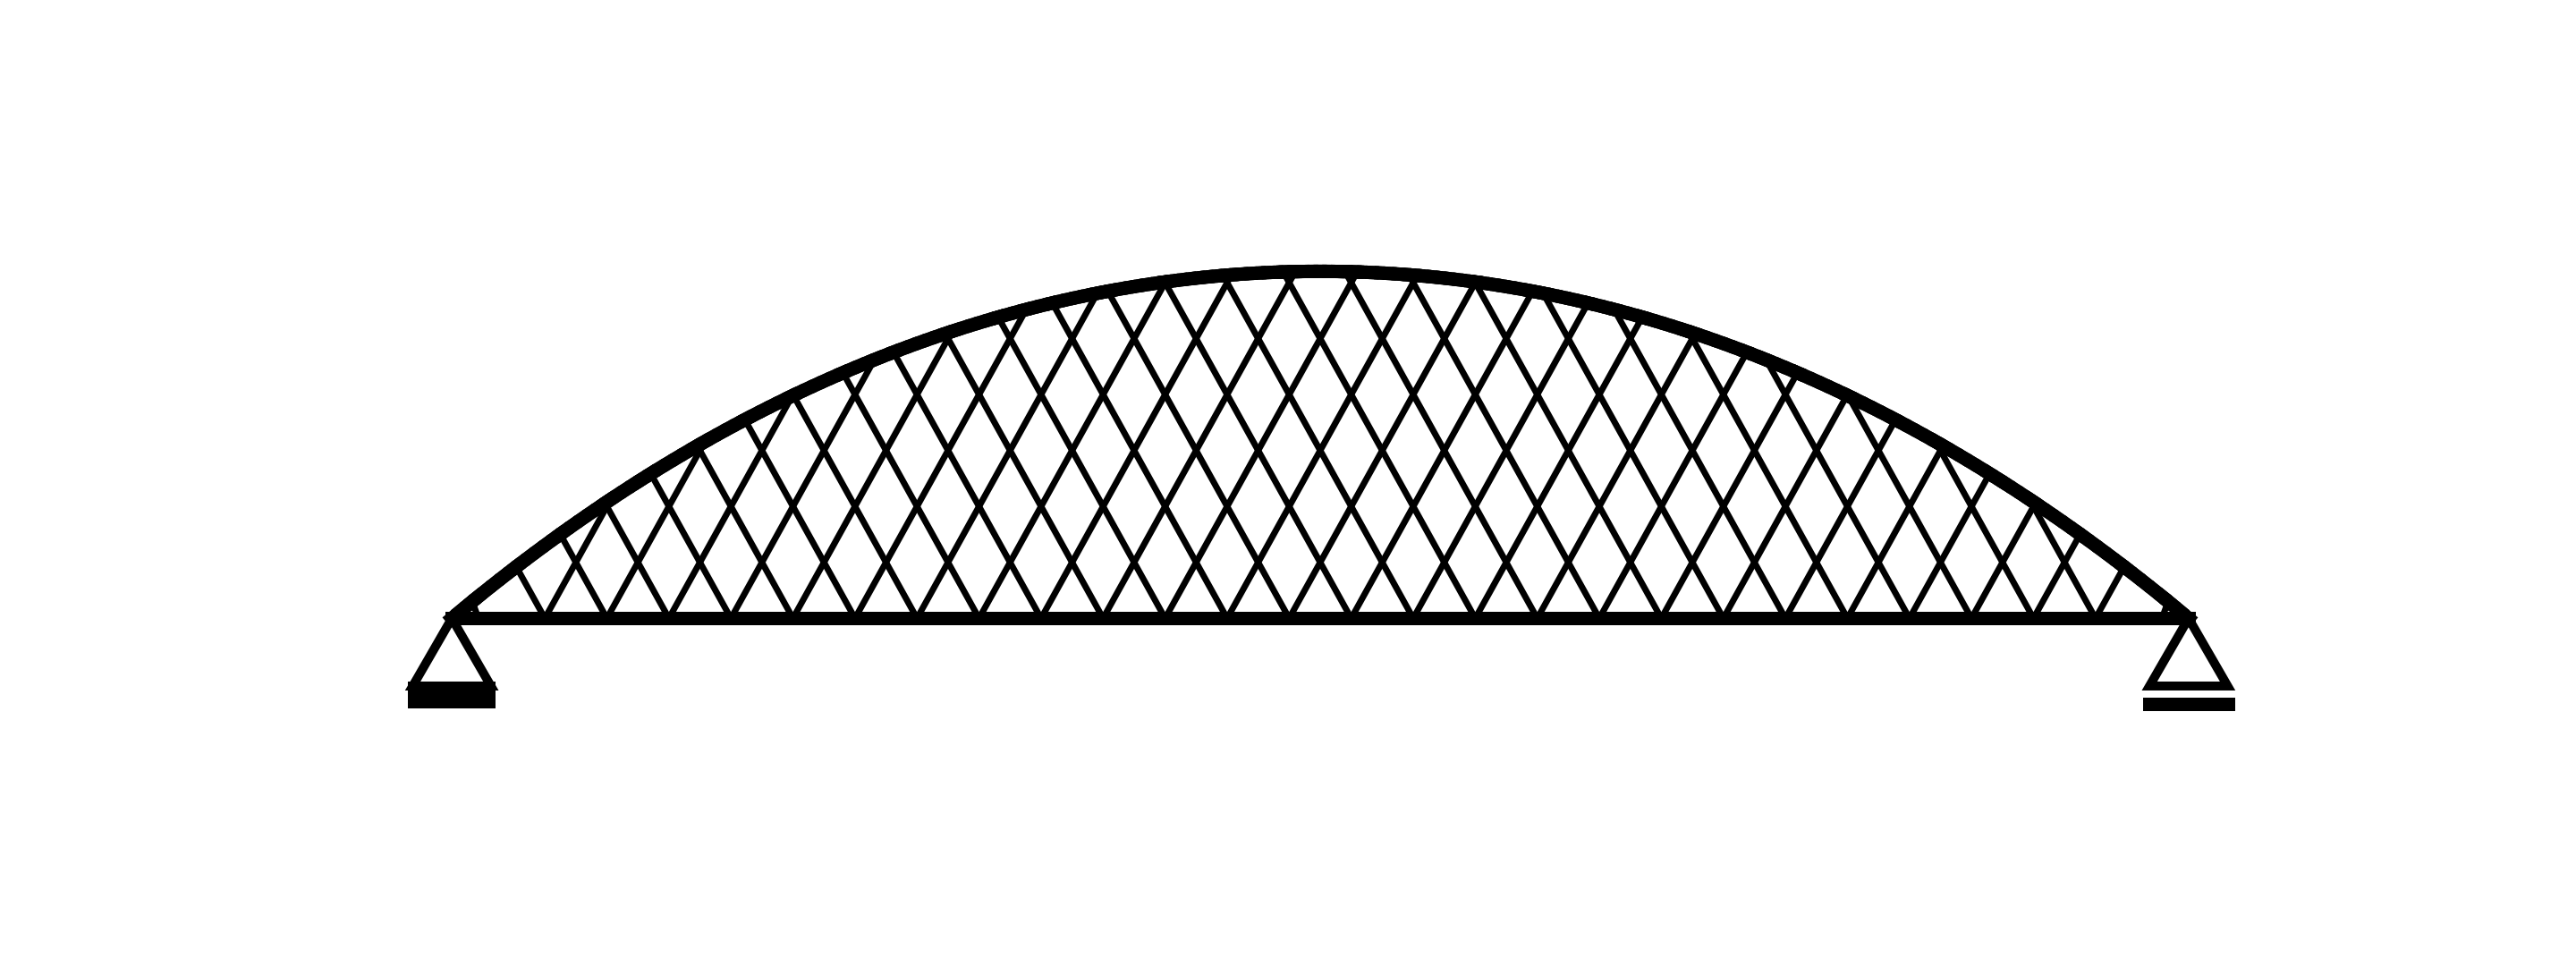
\includegraphics[trim={0 1cm 0 1cm},clip, width=0.65\textwidth]{calculations/hanger amount comparison/structure_26.png}
    \caption{Structural model of a dense hanger arrangement with 26 hangers per set}
    \label{fig:structure_26}
\end{figure}

The optimised effects under permanent loads are shown in Fig \ref{fig:hd_permanent}. As predicted by the investigation of the arch shape, the bending moments in the arch are lowered for an increased hanger density. However, in the knuckle region of the arch the significant bending moments are retained for the dense arrangements. They are due to the tie moment optimisation method assigning significant supernumerary moments to the knuckle. The quartic polynomial approximation is not able to match the corresponding thrust line. The permanent hanger forces are no longer constant for the models with 20 and 27 hangers, as the hangers near the floor beams carry the majority of the forces. At the same time a strong bending moment distribution in the tie is inevitable. The model featuring 26 hangers seems slightly more suitable as it is able to retain constant hanger forces and also a slightly lower tie moment distribution.

\begin{figure}[H]
    \centering
    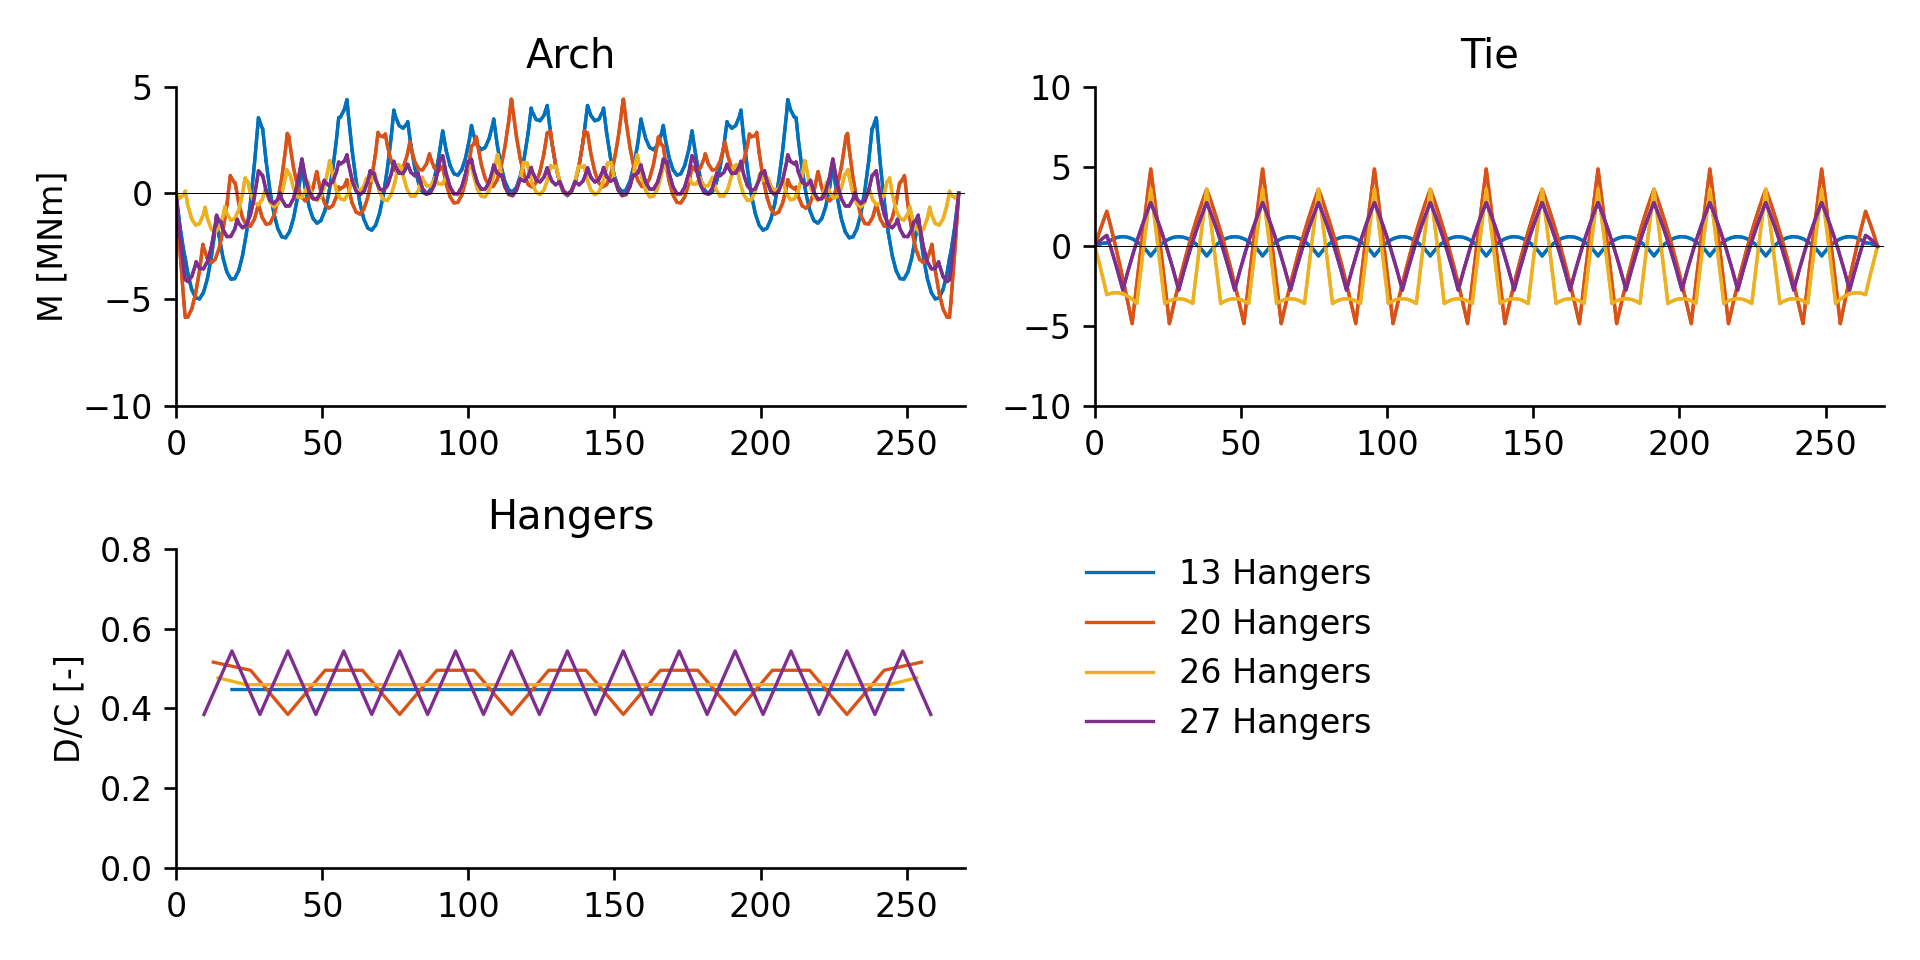
\includegraphics[width=0.75\textwidth]{calculations/hanger amount comparison/permanent state.png}
    \caption{Optimised permanent effects for different hanger densities}
    \label{fig:hd_permanent}
\end{figure}

The elastic responses to dead loading are shown in \cref{fig:hd_elastic_response_dl}.
%On top of the disadvantageous permanent effects, also the elastic response of the modified models to live loading, which are shown in \cref{fig:hd_live}, seem unfavourable.

\begin{figure}[H]
    \centering
    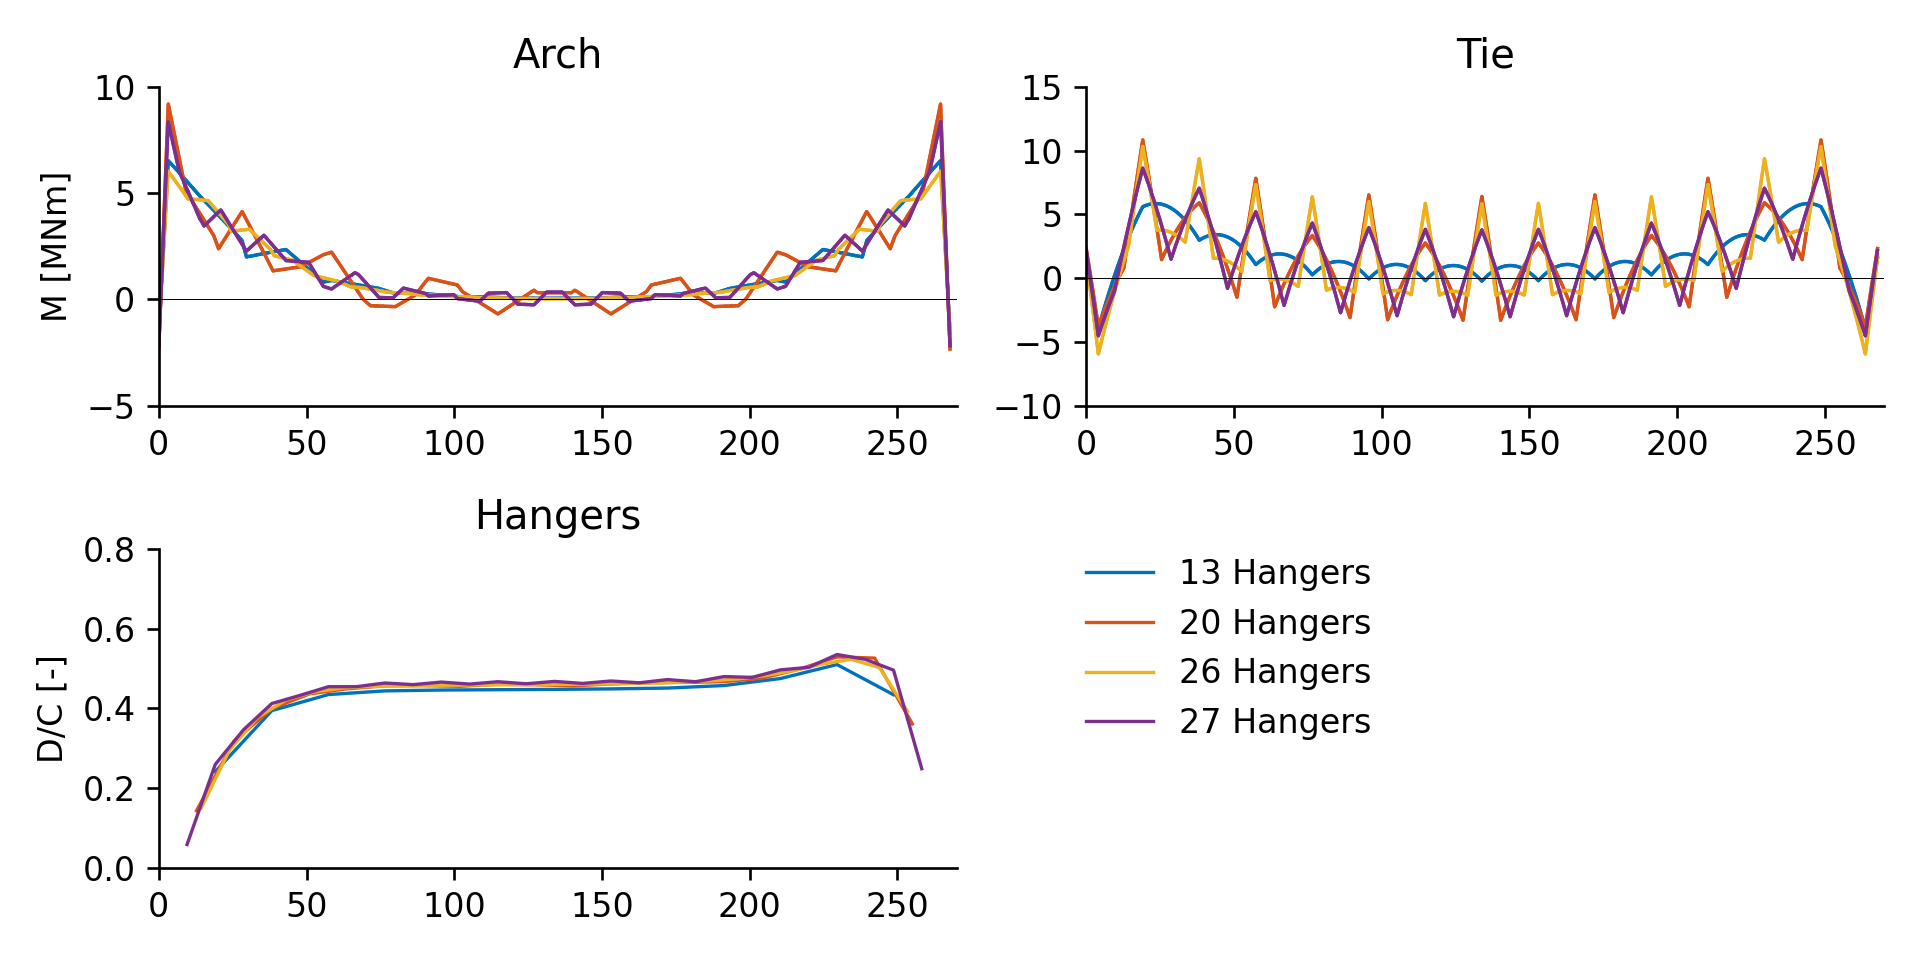
\includegraphics[width=0.8\textwidth]{calculations/hanger amount comparison/dead load.png}
    \caption{Elastic response to dead loading for different hanger densities}
    \label{fig:hd_elastic_response_dl}
\end{figure}

While these effects are already included in the permanent effects, they are still relevant for the design verifications as they are increased or decreased therefor. While the response of the arch and the hangers remains approximately identical, the tie is again affected by stronger bending moments in the denser models. This characteristic is accentuated by the range of tie moments relevant for the tie fracture extreme event, presented in \cref{fig:hd_tie_fracture}.

\begin{figure}[H]
    \centering
    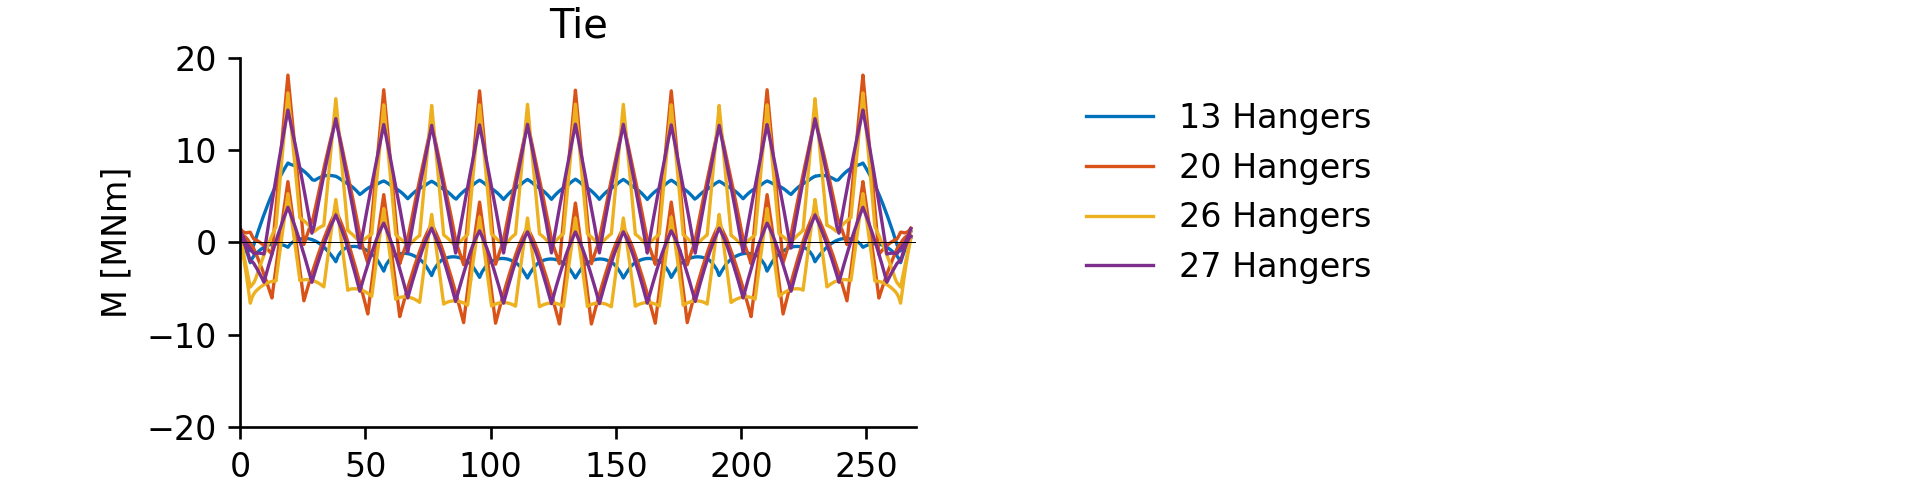
\includegraphics[trim={0 0 3cm 0},clip, width=0.8\textwidth]{calculations/hanger amount comparison/tie fracture.png}
    \caption{Range of tie bending moment for tie fracture extreme event}
    \label{fig:hd_tie_fracture}
\end{figure}

The previously rather uniform moments became particularly peaky. The corresponding design verification in the tie is thereby significantly impaired, as show in Table \ref{tab:hd_dc}. An optimisation of the hanger density itself, therefore renders no potential for optimisation, even though the cable loss extreme event improves as expected.

\begin{table}[H]
    \centering
    \caption{Design verifications for different hanger densities}
    \label{tab:hd_dc}
    \resizebox{0.85\columnwidth}{!}{%
    \input{calculations/hanger amount comparison/dc_comparison.txt}
    }
\end{table}


\section{Floor beam density}
It was seen in the previous chapter, that it is impossible to obtain an optimised design with more hangers per set than floor beams. To facilitate the design verifications in the extreme event of cable loss, a denser hanger arrangement has to be paired with a higher floor beam density. It seems a particularly reasonable step, as the Blennerhassett Island Bridge holds the record for hanger spacing on the tie girder at \SI{20}{m}. This was only feasible as the extreme event of floor beam loss was not considered in the design. However, there are other causes to investigate the floor beam and hanger density. Besides the previously mentioned improved behaviour under cable loss and smaller deviations of the arch from the thrust line, a general more continuous transfer of loads might be beneficial. \medskip

Theoretically, an adapted floor beam spacing changes the entire deck system and its weight. However, the deck is not subject to this investigation and it is therefore assumed, that the total weight of the deck system and the floor beams is constant and independent of the floor beam spacing. Four models with different floor beam and hanger densities are investigated in this Section. Besides the final design with 13 floor beams, models with 10, 20 and 27 floor beams are investigated. As an advantage for the sparse model with 10 floor beams, the actual thrust line is assumed as the arch shape. For the other models, the thrust line is approximated by the quartic polynomial. The respective permanent effects are shown in \cref{fig:fb_permanent}.

\begin{figure}[H]
    \centering
    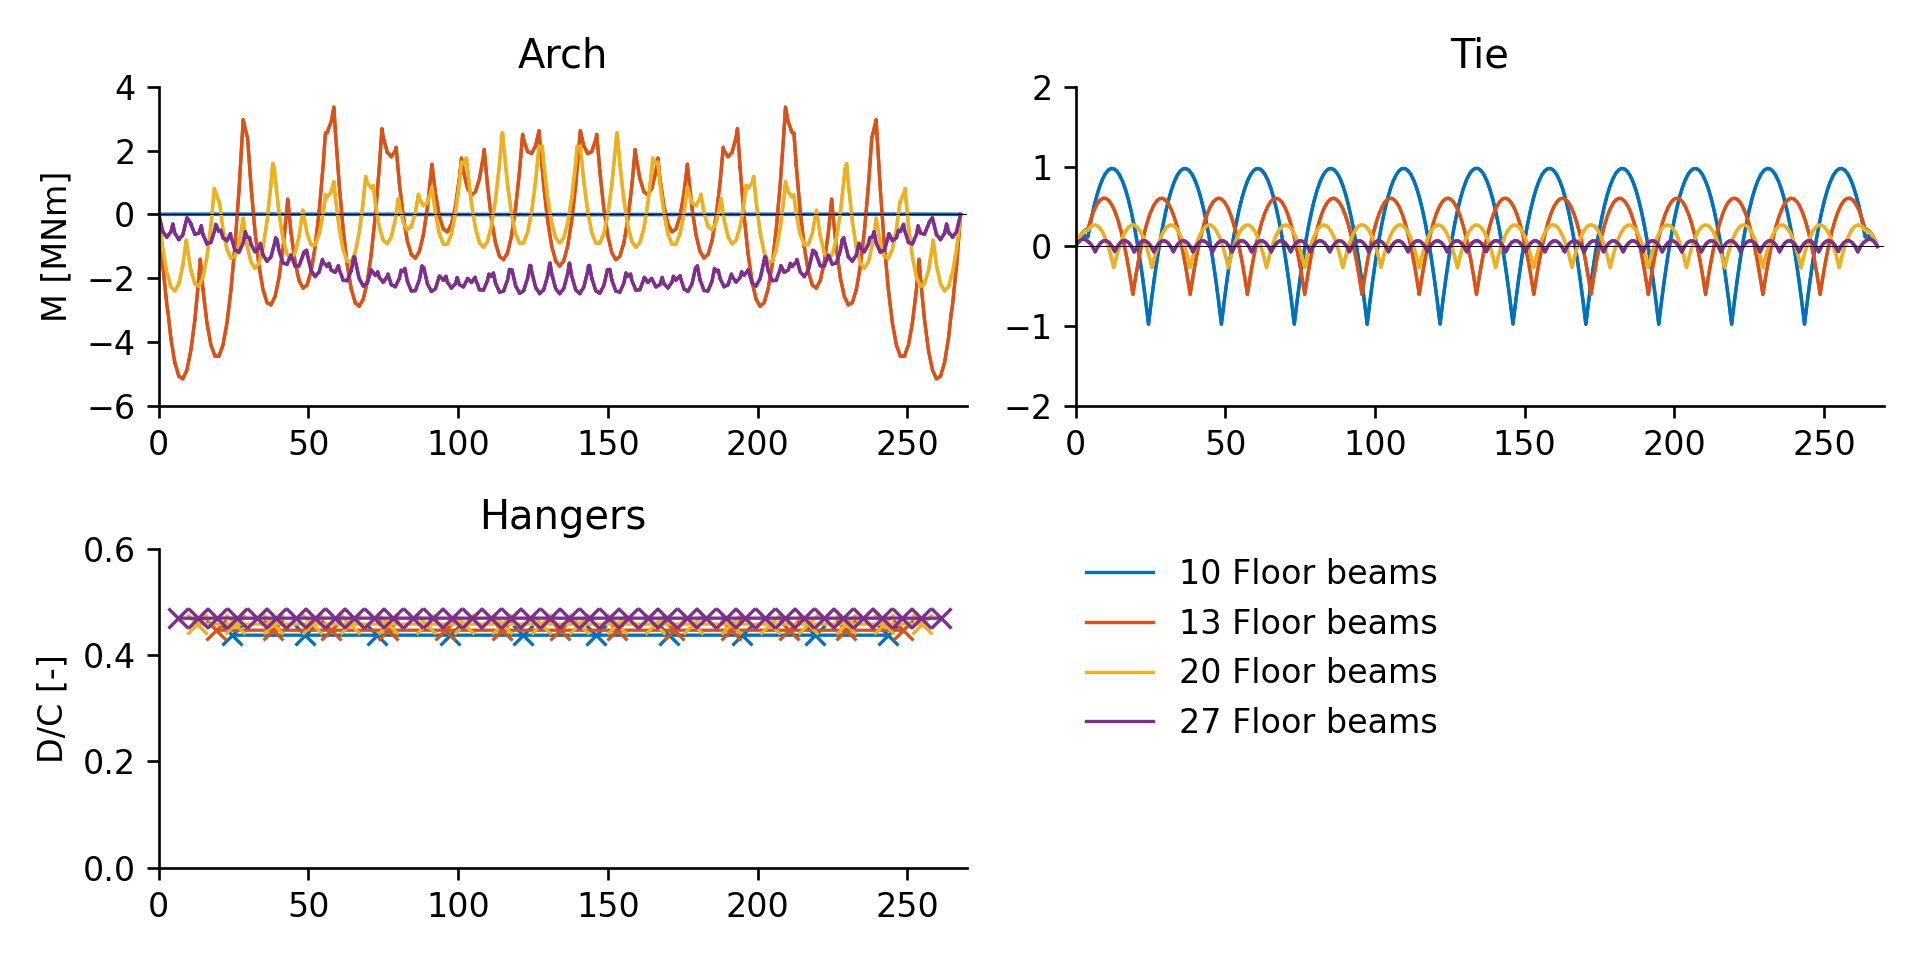
\includegraphics[width=0.8\textwidth]{calculations/floor beam comparison/permanent state.png}
    \caption{Optimised permanent effects for different floor beam densities}
    \label{fig:fb_permanent}
\end{figure}

All models retain the characteristic permanent effects resulting from the tie optimisation, which are the uniform hanger forces and a uniform tie moment distribution with peaks at $M=\pm\,g_{Tie} \cdot s^2 / 16$. It can be seen, that the hanger forces slightly increase, as less weight of the deck is directly carried by the floor beam at the knuckle. Compared to the other models, the permanent arch moments for 13 floor beams seem to be significant. However, it is known from the investigation of the arch shape, that the moments only lower the demand over capacity ratio by about 0.05. \medskip

In \cref{fig:fb_live} the elastic response under characteristic live loading is shown. For the hangers, the response is practically unchanged. Only the hangers very close to the knuckle undergo a lower normal force, as the tie girder at the knuckle carries the corresponding load directly to the knuckle. For the tie girder, the moment effects increase with the floor beam density and constitutes a slightly impairing impact on the design verifications. The stronger moments are due to the weaker coupling of the tie and the arch at the floor beams. While the force at the floor beams for the distributed lane load decreases, the force of the design trucks remain the same. They are responsible for the slightly increased hanger forces and bending moments in the tie girder. The moment distribution on the arch rib shows a different tendency. Overall the effects of the models resemble a similar shape. However, for fewer floor beams, certain moment peaks due to the stronger hanger forces become apparent. To put these differences into the context of the design verifications, the resulting demand over capacity ratios are shown in Tab. \ref{tab:fb_dc}.

\begin{figure}
    \centering
    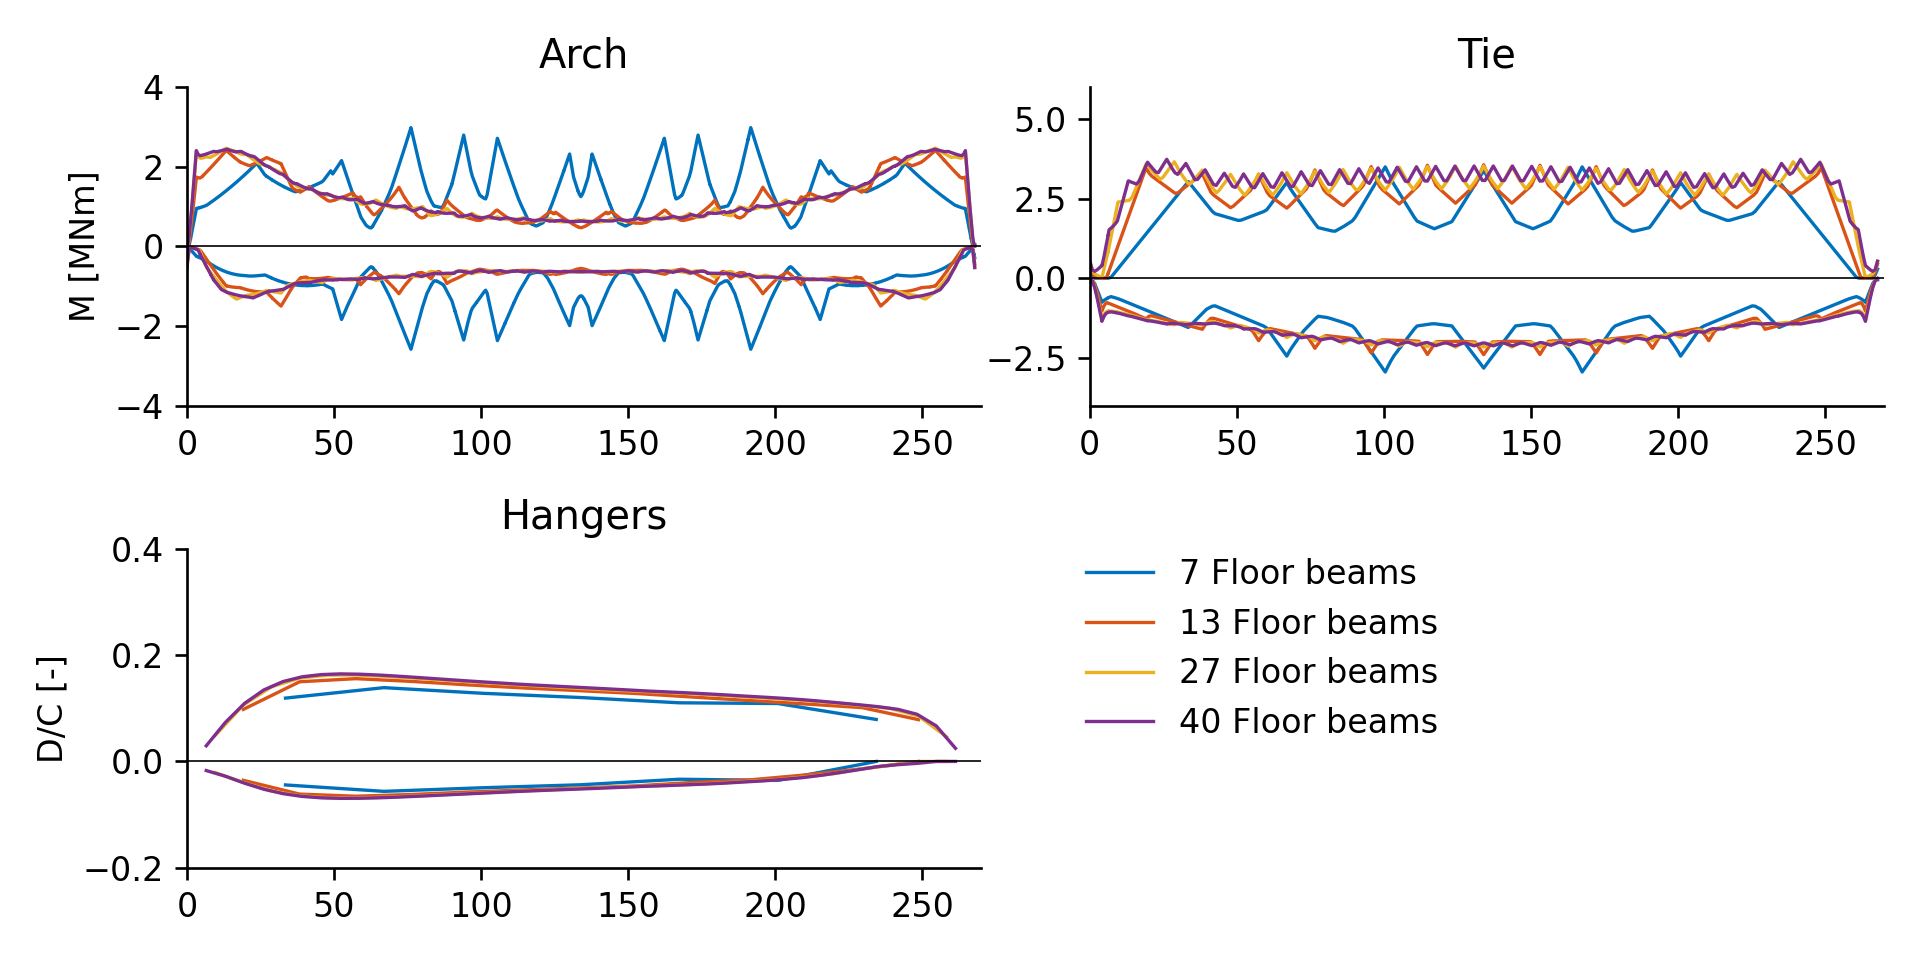
\includegraphics[trim={0 0.4cm 0 0.4cm},clip, width=0.78\textwidth]{calculations/floor beam comparison/live loading.png}
    \caption{Elastic effects under live loading for different floor beam densities}
    \label{fig:fb_live}
\end{figure}

\begin{table}[H]
    \centering
    \resizebox{\columnwidth}{!}{%
    \input{calculations/floor beam comparison/dc comparison.txt}
    }
    \caption{Design verifications for different floor beam densities}
    \label{tab:fb_dc}
\end{table}

The extreme event of cable loss is well controlled by a denser hanger arrangement, as was already observed in the previous chapter. The impacts on the other design verification are comparably small. Both the hangers and the tie girder undergo a decrease of about 0.05 in the demand over capacity ratio. The effect ranges for the strength-I limit state are shown in \cref{fig:fb_strength} for further details. Considering the arch, 10 floor beams with an optimised shape or 27 floor beams show a well balanced moment distribution. However, also the moments in the other models do not have a decisive influence on the design.

\begin{figure}[H]
    \centering
    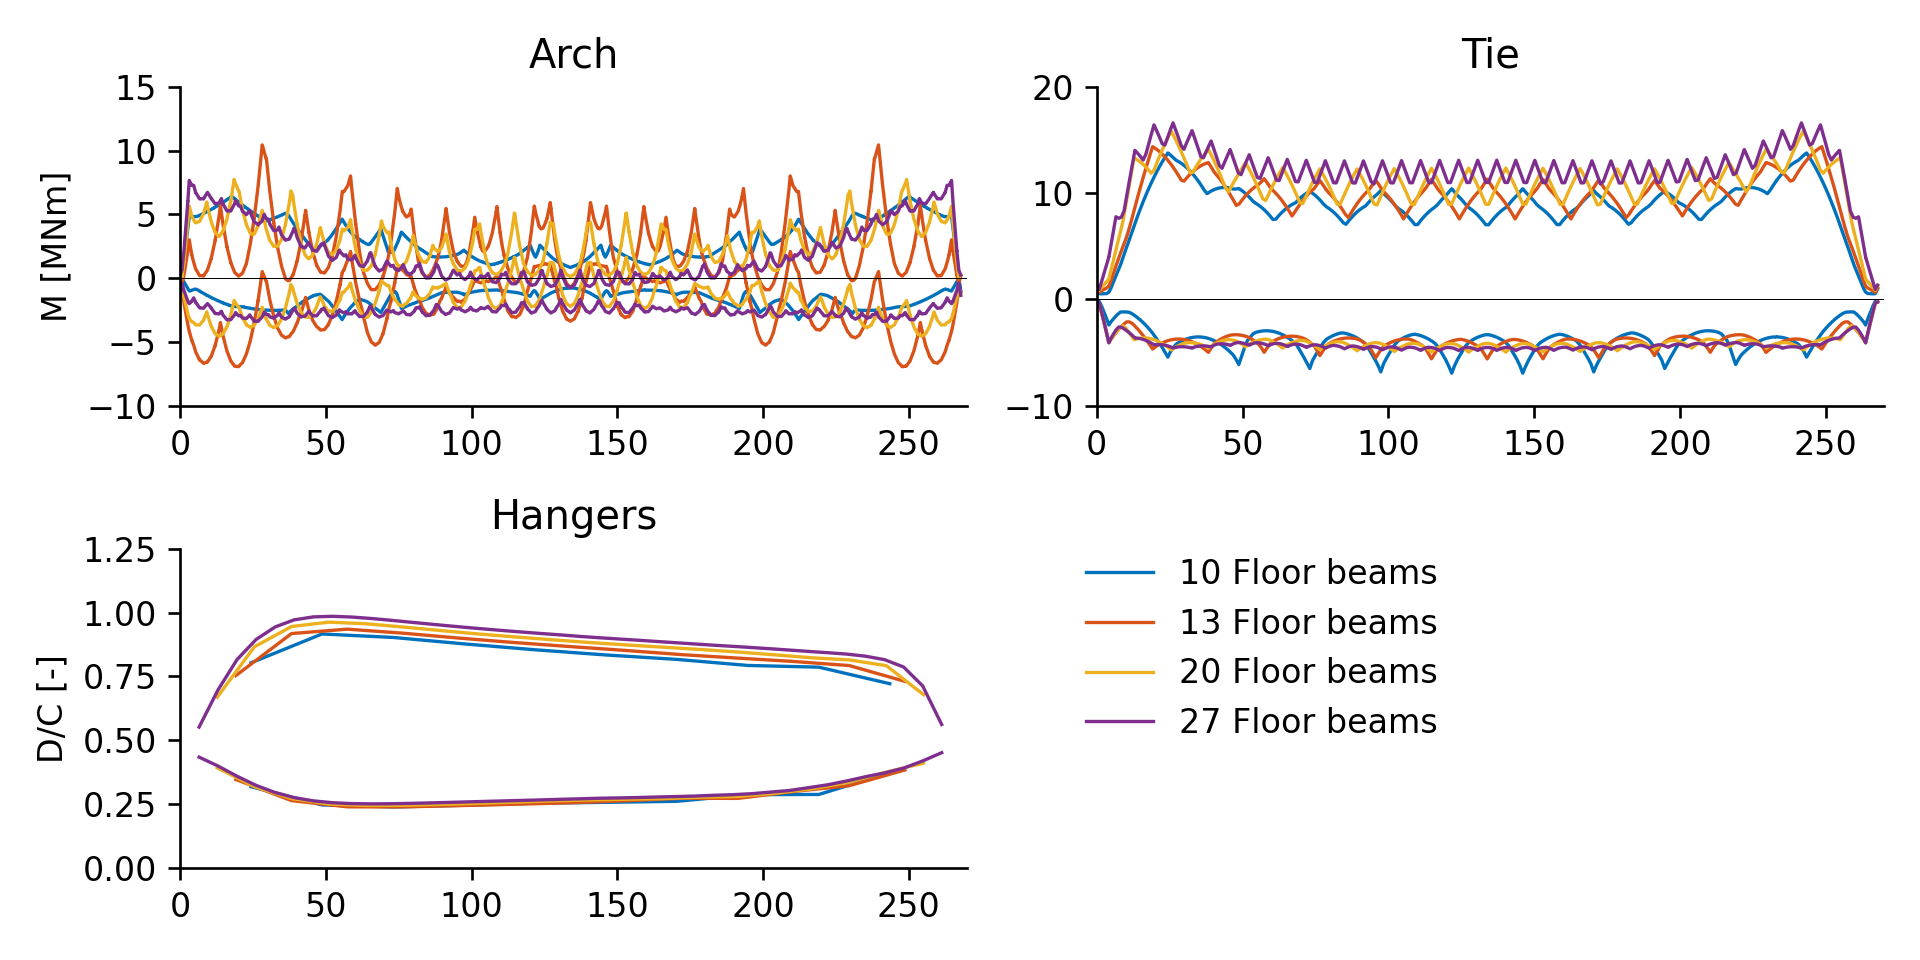
\includegraphics[trim={0 0.4cm 0 0.4cm},clip, width=0.78\textwidth]{calculations/floor beam comparison/strength-I.png}
    \caption{Strength-I effects for different floor beam densities}
    \label{fig:fb_strength}
\end{figure}

[Beschreibung des Kostenverlaufs]

\begin{figure}[H]
    \centering
    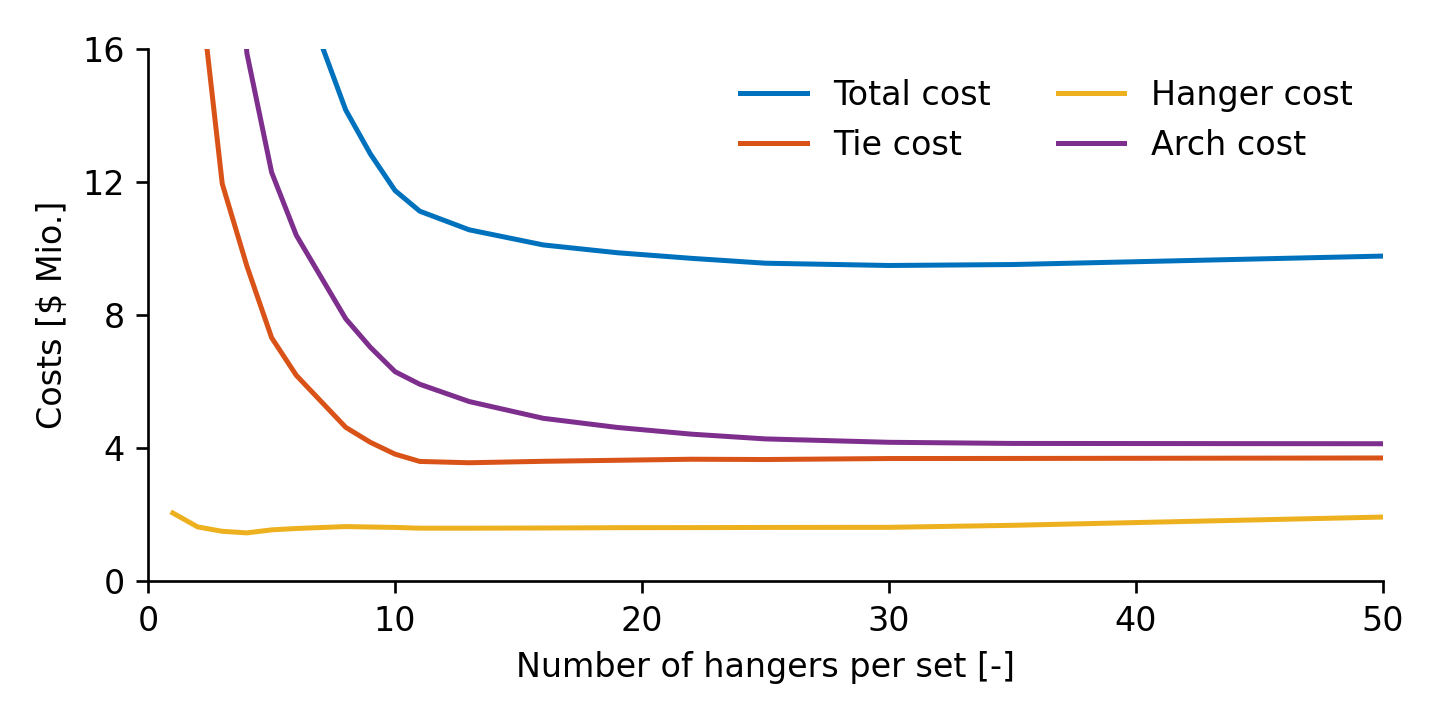
\includegraphics[width=0.7\textwidth]{calculations/floor beam comparison/cost comparison.png}
    \caption{Estimated costs for different floor beam densities}
    \label{fig:fb_costs}
\end{figure}


\newpage
\section{Hanger inclination}
The investigation in this section focuses on the parallel hanger arrangement's main parameter, the hanger inclination. In the previous Sections, the inclination has been left at \SI{64}{\degree} as in the final design of the Blennerhassett Island Bridge. This choice is critically assessed by the investigation of models with inclinations from \SI{45}{\degree} to \SI{85}{\degree}. In a first part, it is focused on their elastic response to the characteristic load cases and the internal forces under permanent loads.  In a second part, the implications on the design verification and the estimated costs are examined. To conclude this section, variable hanger inclinations are considered. Therefore, the constant change of inclination arrangement is investigated for further optimisation potential.


\subsection{Parallel hanger arrangement}
\subsubsection{Characteristic behaviour}
The investigation of the arch shape in Section \ref{sec:arch_shape}, showed that the spacing of the hanger anchorage nodes on the arch rib has a significant impact on the internal forces for the considered design. By changing the inclination of the hangers the respective spacing changes rather randomly. To exclude these random implications in this investigation of the hanger inclination, the arch shapes are taken as the respective thrust lines of each arrangement. Hence, the permanent moment distributions disappear for all models. Also the permanent moment distribution on the tie girder resulting from the tie moment minimisation is identical for all models at $M_{p,Tie}=\pm \SI{650}{kNm}$. The other permanent internal forces are shown in \cref{fig:inclination_permanent}.

\begin{figure}[H]
    \centering
    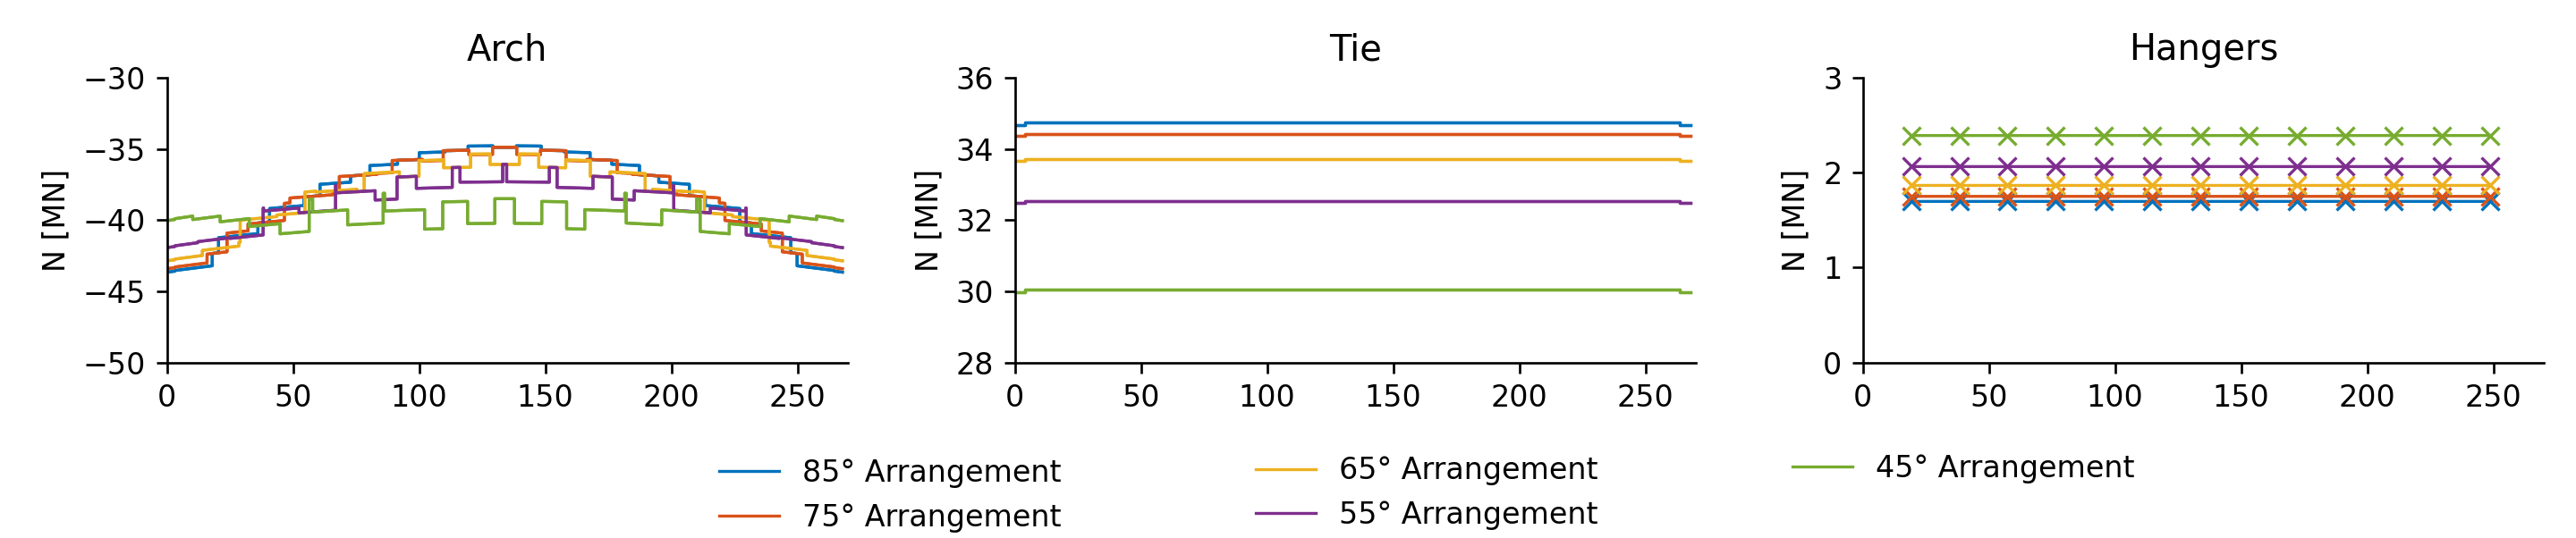
\includegraphics[trim={1cm 0 1cm 0},clip, width=\textwidth]{calculations/parallel arrangement comparison/permanent_plot.png}
    \caption{Permanent internal forces for different hanger inclinations}
    \label{fig:inclination_permanent}
\end{figure}

The permanent hanger forces increase for flatter hanger inclinations due to the smaller vertical component of the respective force. For each model they are still uniform and cause no change in the normal force distribution in the tie girder. For the normal forces in the arch, a rather uniform distribution is observed for the \SI{45}{\degree} arrangement. For the respective continuous hanger arrangement, it was seen in \cref{sec:arch_shape}, that its thrust line resembles a circle and the hanger forces on the arch are oriented radially. Therefore, the direction of the resulting normal force changes, the magnitude remains the same however. Apparently, this behaviour also applies to the considered discrete \SI{45}{\degree} arrangement. Its lower normal force at the knuckle can alternatively be explained by the steeper inclination of the circle, which approximates the thrust line of the flat arrangements. As the vertical component of the normal force in the arch is roughly the same for all models, the total normal force is smaller for steep arch shapes at the knuckle. Conversely, the \SI{45}{\degree} arrangement causes a higher normal force in the crown of the arch. This high normal force is due to the horizontal force components in the hangers, which reduces the structure's global lever arm and also the tension in the tie. 
A similar elastic response is observed for the characteristic dead loading, shown in \cref{fig:inclination_dead}.
\begin{figure}[H]
    \centering
    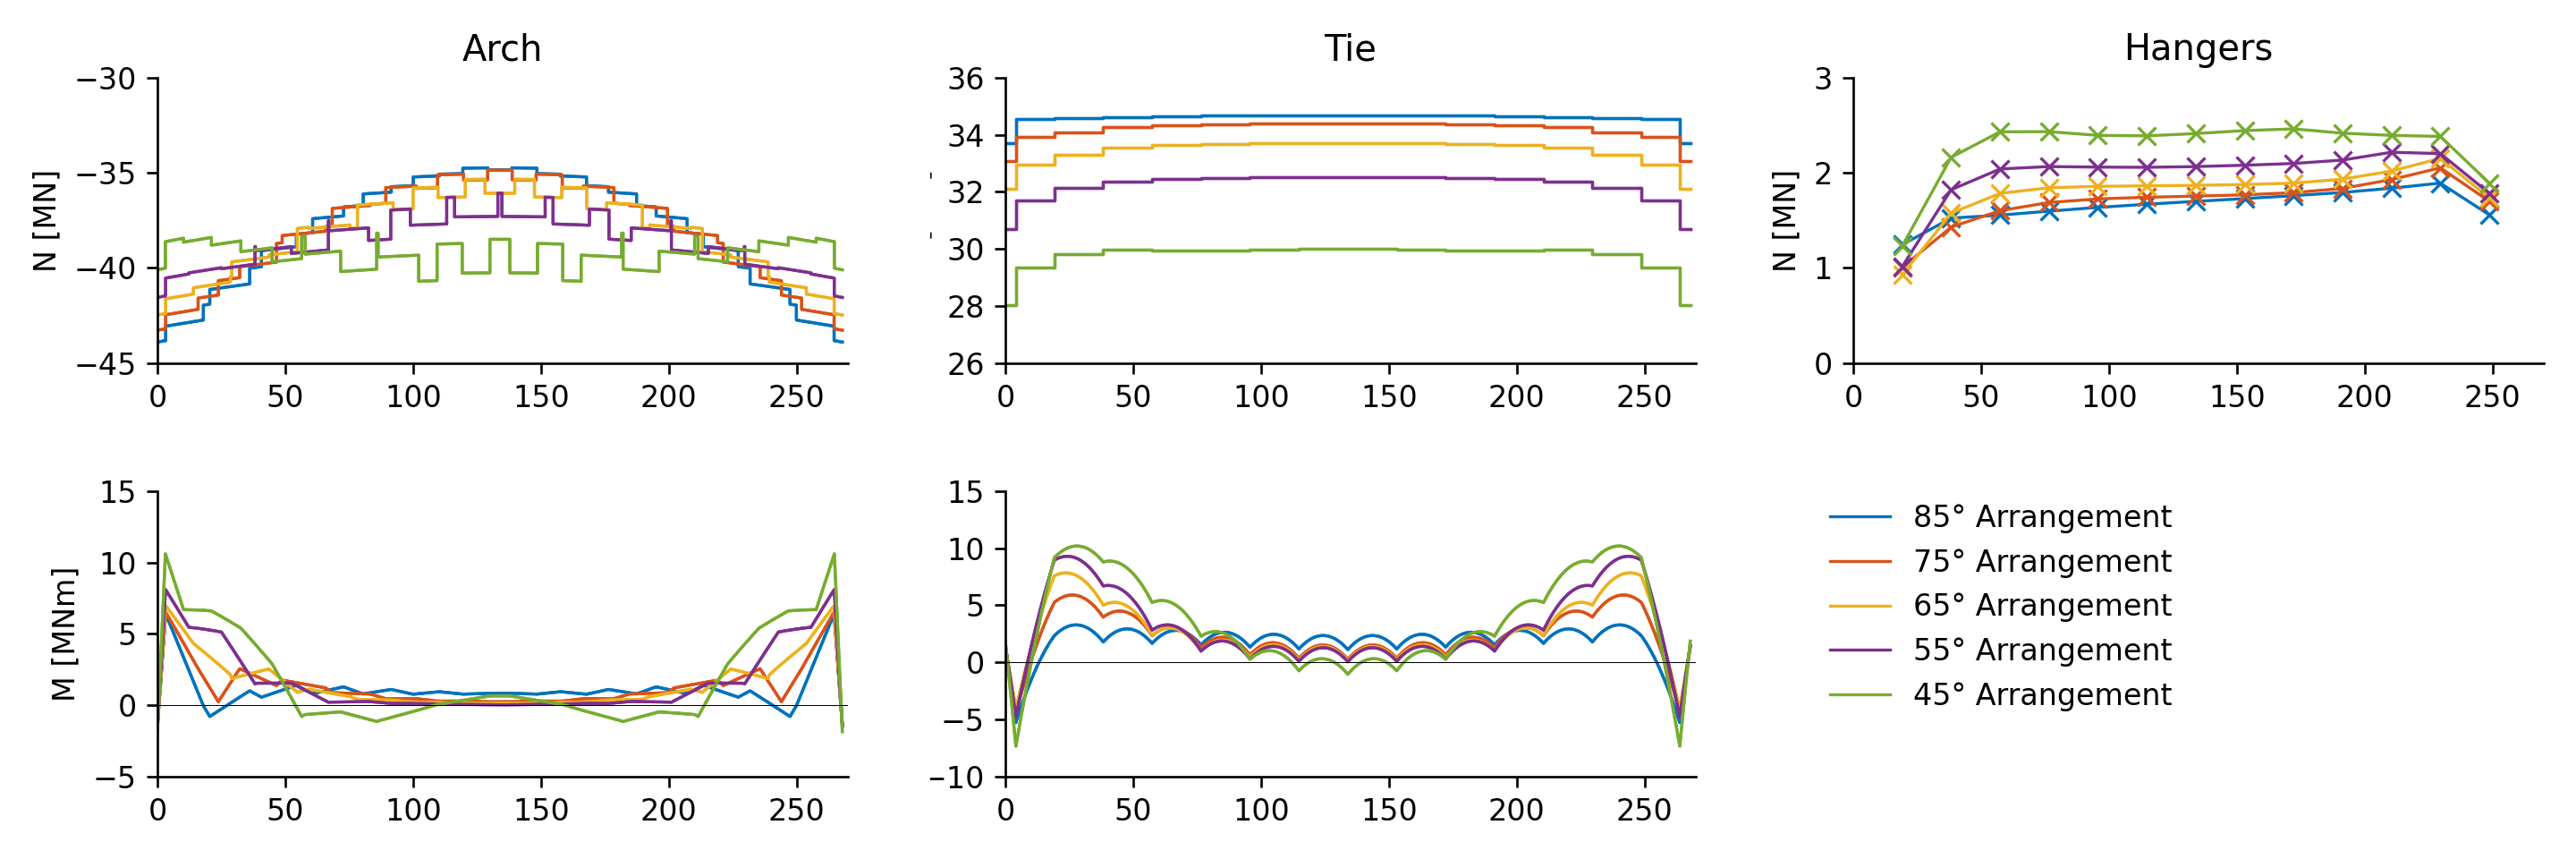
\includegraphics[width=0.95\textwidth]{calculations/parallel arrangement comparison/dead load_plot.png}
    \caption{Elastic responses to dead loading for different hanger inclinations}
    \label{fig:inclination_dead}
\end{figure}

Most hanger forces are in a similar range as for the optimised permanent state. This is due to the uniform embedding of the tie girder in the field yielding uniform hanger forces. Therefore, also the normal forces of the arch and the tie show a similar shape as was seen for the permanent state. However, in the knuckle area large bending moments are observed for flat inclinations. Their cause is the lack of stiffness between the arch and the tie in this region, leaving them to carry the loads on bending. This lack of stiffness becomes obvious from the respective hanger arrangements presented in \cref{fig:arrangements}.

\begin{figure}[H]
\centering
\begin{subfigure}{0.5\textwidth}
    \centering
    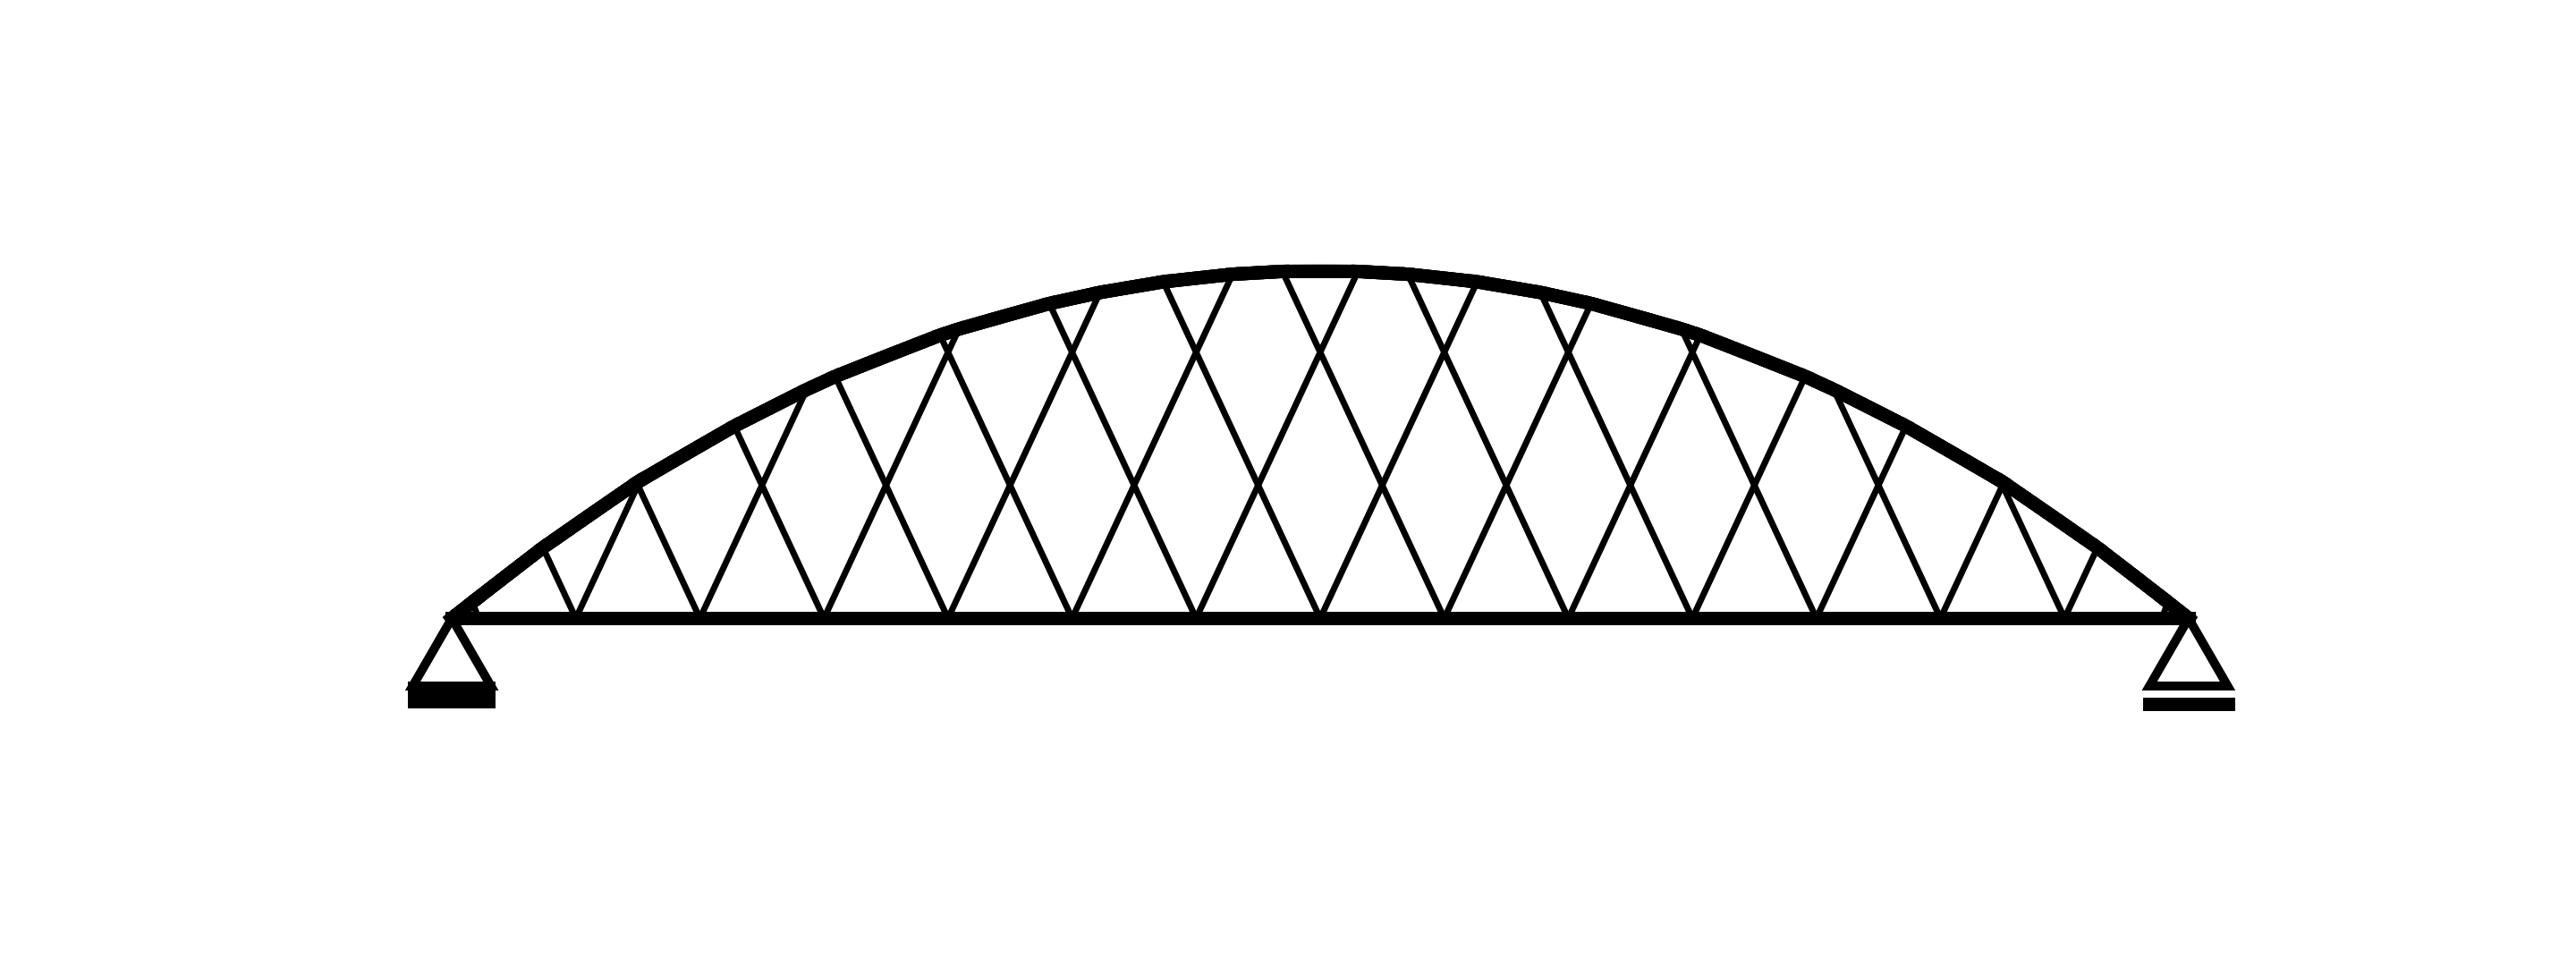
\includegraphics[trim={40 25 189 40},clip, width=0.5\textwidth]{calculations/parallel arrangement comparison/arrangement_65.png}
    \caption{65\degree Arrangement}
    \label{fig:arrangements_65}
\end{subfigure}%
\begin{subfigure}{.5\textwidth}
    \centering
    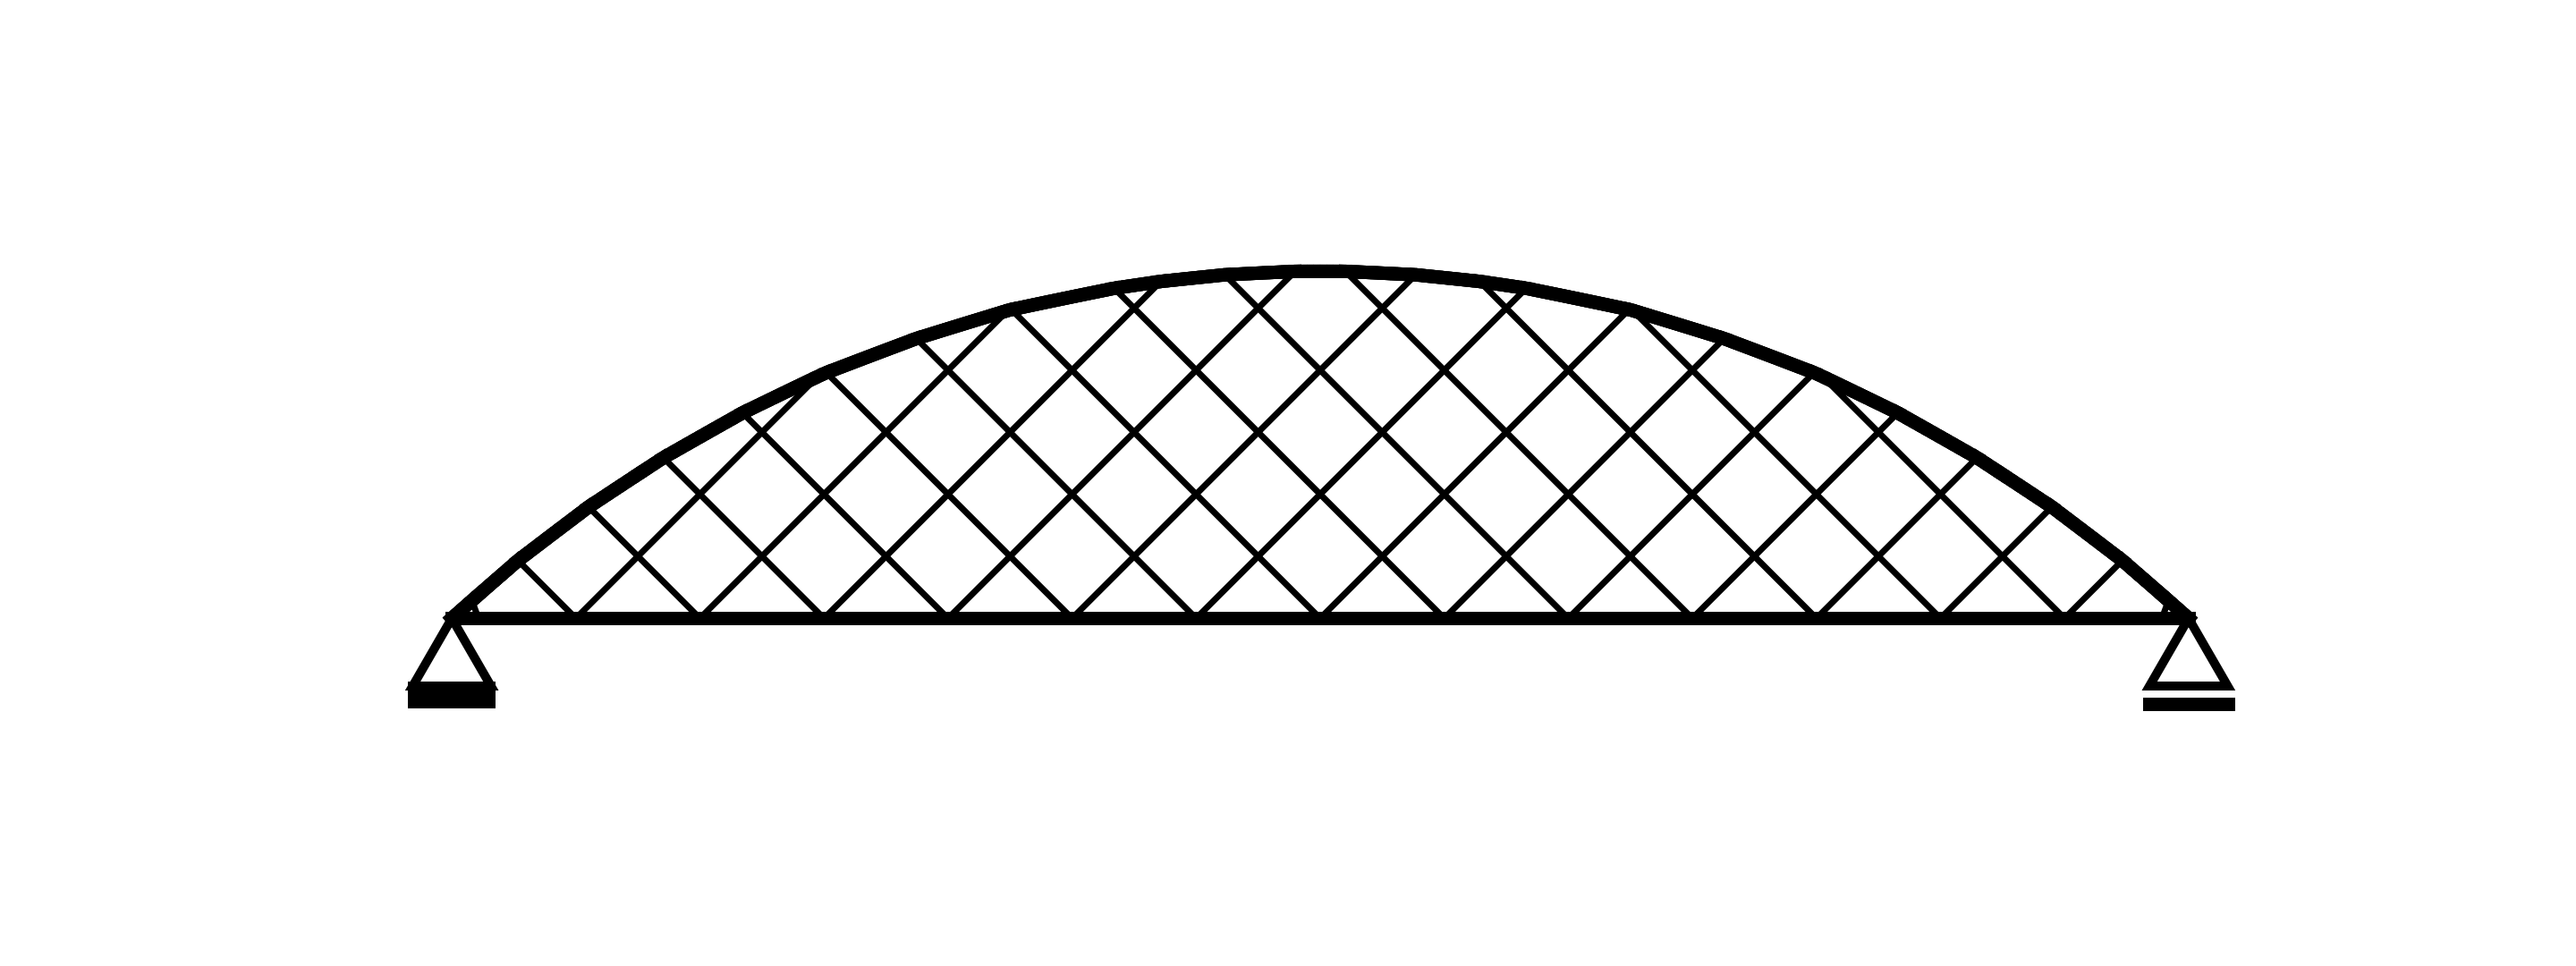
\includegraphics[trim={40 25 189 40},clip, width=0.5\textwidth]{calculations/parallel arrangement comparison/arrangement_45.png}
    \caption{45\degree Arrangement}
    \label{fig:arrangements_45}
\end{subfigure}
\caption{The knuckle region for different hanger inclinations}
\label{fig:arrangements}
\end{figure}

The \SI{45}{\degree} arrangement features only hangers from one set in the knuckle region, which additionally attach almost perpendicular to the arch. The stiffness of this arrangement is therefore much lower than the one of the \SI{65}{\degree} arrangement, which has more connections and also more suitable hanger inclinations. Further, the elastic response range to live loading is presented in \cref{fig:inclination_live}.

\begin{figure}[H]
    \centering
    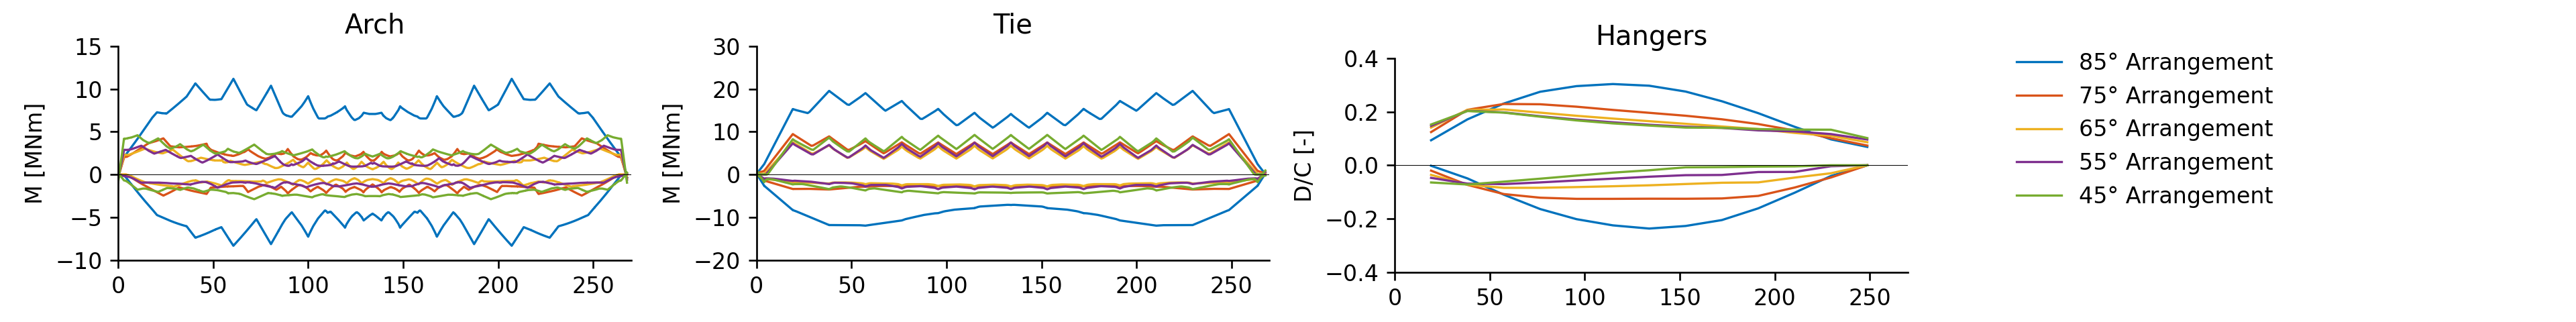
\includegraphics[trim={1cm 0 1cm 0},clip, width=\textwidth]{calculations/parallel arrangement comparison/live loading_plot.png}
    \caption{Elastic response ranges to live loading loading for different hanger inclinations}
    \label{fig:inclination_live}
\end{figure}

For live loading, it is the steepest arrangement which is affected by the largest internal force effects. Especially its hanger force shows a unique behaviour with the ones in the middle carrying the largest forces. As the hangers are less interconnected with each other the coupling of the arch and the tie is generally lower. Therefore, the \SI{85}{\degree} arrangement is affected by larger bending moments, as the efficient truss action is not formed. Further, this increases the characteristic length of the embedded tie girder, which especially causes the middle hanger to be affected by large forces. There can also be strong compressive forces for the considered hanger, which implicates the danger of hanger unloading. However, it has to be considered that the steep hanger arrangement utilises a shorter total hanger length, which poses an upside opposing the observed disadvantages. Within the other four studied models the differences are much lower. Still, it is indicated by the lower moment distributions for the \SI{55}{\degree} and the \SI{65}{\degree} arrangements, that a stronger truss action is formed in the respective cases. It can be concluded, that neither a steep nor a flat hanger arrangement forms an adequate coupling of the arch rib and the tie girder. 
Ultimately, the effects for the event of losing the fourth cable are shown in \cref{fig:inclination_cable} to representing the charcteristic behaviour under cable loss.

\begin{figure}[H]
    \centering
    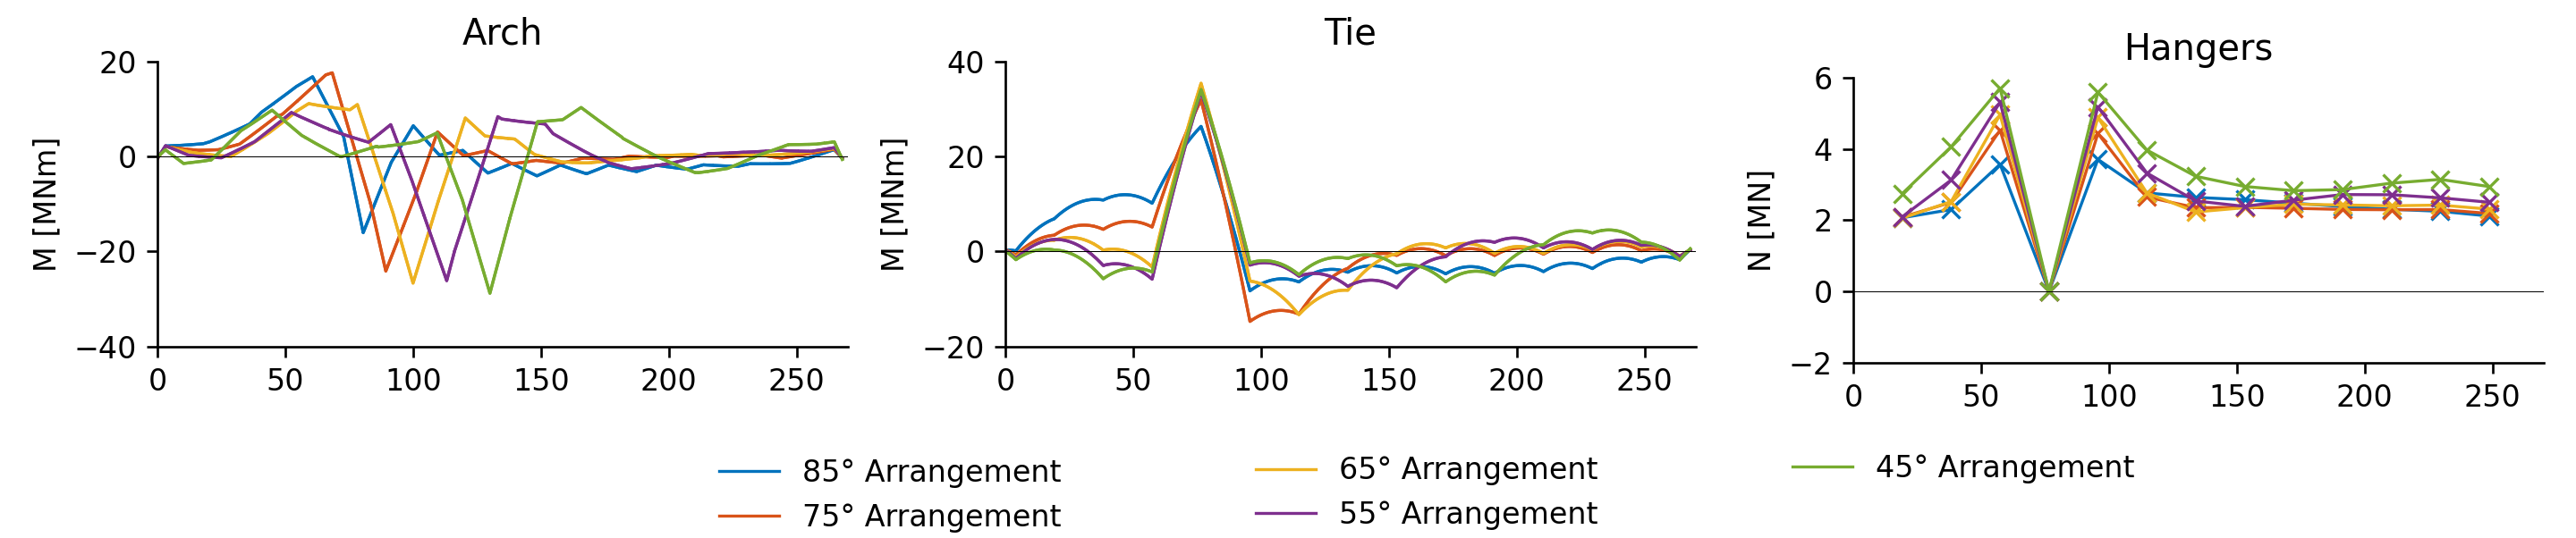
\includegraphics[trim={1cm 0 1cm 0},clip, width=\textwidth]{calculations/parallel arrangement comparison/cable loss 4_plot.png}
    \caption{Approximated dynamic response to the loss of the fourth hanger for different hanger inclinations}
    \label{fig:inclination_cable}
\end{figure}

The extreme event of cable loss shows again the opposite tendency. Because of the generally lower permanent hanger forces and the weaker coupling, the steep arrangements result in lower demands compared to the flat inclinations. Further, the similar directions of the two hanger sets allows them to better distribute the forces of the lost cable. 

\subsubsection{Design verifications and costs}
To conclude the previous observations, the deciding demand over capacity ratios are shown for each model and reach segment in Table \ref{tab:dc_inclination}.

\begin{table}[H]
    \centering
    \caption{Maximum demand over capacity ratios for different hanger inclinations}
    \label{tab:dc_inclination}
    \resizebox{\columnwidth}{!}{%   
    \input{calculations/constant change arrangement/dc_comparison.txt}
    }
\end{table}
In the arch segments, a decrease for the demand in the extreme event of cable loss is observed for steeper arrangements. It is mainly due to the significant horizontal components in the flat arrangements. While the normal force under identical vertical components is approximately 40\% greater for the \SI{45}{\degree} arrangement, the demand is approximately 20\% larger, as not the entire demand results from the lost normal force. On the other hand, the verification slightly improves for the first arch segment, due to the lower normal force in the knuckle region. For the segments on the tie girder the extreme event of tie fracture remains decisive for all models. The large increase in demand for the steepest arrangement is due to its inefficient behaviour under live loading. Between the other models, it is the lower normal force in the tie girder which renders the flat arrangement slightly beneficial. For hangers, neither of the extreme arrangements gives an improvement. The steep hanger arrangement suffers from fatigue due to the weak interconnection between the hangers. For the flat arrangement it is again the cable loss event which causes the highest demands. An optimum demand for the hangers is obtained by the \SI{65}{\degree} and the \SI{75}{\degree} arrangement. Finally, the costs of the investigated models, which are shown in \cref{tab:cost_inclination}, are considered. Correlating to the previous observations, the costs of the arch rib can be reduced by steeper arrangements, whereas the tie girder becomes cheaper for flat inclinations. Significant changes are also observed for costs of the hangers which are optimised for inclinations similar to the final design. Also the overall costs are minimised for these models. However the optimum range is rather broad from \SI{65}{\degree} to \SI{75}{\degree}.


\begin{table}[H]
    \centering
    \caption{Maximum demand over capacity ratios for different hanger inclinations}
    \label{tab:cost_inclination}
    \input{calculations/constant change arrangement/cost_comparison.txt}
\end{table}


\subsection{Constant change of inclination arrangement}

\subsection{Unpatterned arrangement}



\section{Summary}











